% !TEX root = SegwayDoku.tex


% tragt hier eure Unterdokumente in der Reihenfolge ein,
% in der sie im Gesamtdokument auftauchen sollen

% !TEX root = SegwayDoku.tex
\renewcommand{\autoren}{Stephan Morongowski}
\newpage
\section{Definition eines roboterfesten Koordinatensystems}

\begin{figure}[h]  % [h] bedeutet, dass das Bild genau an dieser Stelle im Text erscheint
\centering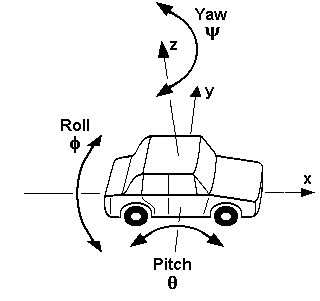
\includegraphics[width=0.6\textwidth]{images/FahrzeugKSys_mod.png}
\caption[Roboterkoordinatensystem]{Roboterkoordinatensystem \newline (Quelle: \cite{roboterKS_Bild})}
\label{robotKSys}
\end{figure}

Zur einheitlichen Bezeichnung wurde das roboterfeste Koordinatensystem (im Folgenden mit KS bezeichnet) wie in Abbildung \ref{robotKSys} zu sehen, ähnlich ISO 88551 festgelegt. Entgegen der häufig anzutreffenden Bezeichnungen der Winkel um die jeweiligen Koordinatenachsen werden im Folgenden die Winkel um
\begin{itemize}
    \item die x-Achse mit \(\alpha\)
    \item die y-Achse mit \(\beta\)
    \item die z-Achse mit \(\gamma\)
\end{itemize}
bezeichnet. \\
Der Ursprung des KS liegt auf der Radachse mittig zwischen den beiden Rädern.\\
Das KS ist ein rechtshändiges KS.\\\\
Die Verdrehung der jeweiligen Räder wird mit \(\varphi_l\) bzw. \(\varphi_r\) bezeichnet. Dabei bezeichnet \(l\) das in positive x-Richtung blickend links liegende Rad und \(r\) das in positive x-Richtung blickend rechts liegende Rad.

\newpage

% !TEX root = ../SegwayDoku.tex
%\renewcommand{\autoren}{Stephan Morongowski}
\newpage

\section{Umsetzung eines Direktantriebes}

% !TEX root = ../SegwayDoku.tex
\renewcommand{\autoren}{Severin Schendel	}
%\newpage
\subsection{Vergleich der Antriebsarten}
\subsubsection{Bürstenloser Gleichstrommotor}

\begin{quote}
"Bürstenlose Gleichstrommotoren, kurz BLDC („Brushless DC-Motoren), sind -  entgegen ihrer Bezeichnung - Drehstrom-Synchronmaschinen: Der Läufer folgt einem magnetischen Drehfeld, die Bewegung ist synchron zur Wechselspannung, die an die Wicklungen angelegt wird. Dieser Motortyp wird häufig als „Bürstenloser Gleichstrommotor“ bezeichnet, da er in vielen Applikationen bürstenbehaftete Gleichstrommotoren („brushed DC“, Kommutatormotoren) ersetzt. Bei einem bürstenbehafteten Gleichstrommotor wird eine Gleichspannung angelegt, die durch einen mechanischen Wechselrichter im Motor - die Bürsten - einen drehzahlunabhängigen Wechselstrom erzeugt.

Zusammen mit einer elektronischen Ansteuerung, die die Funktion der Bürsten übernimmt und aus den eingespeisten Gleichstrom in Wechselstrom umwandelt, entspricht der BLDC-Motor im Verhalten einem bürstenbehafteten Gleichstrommotor ohne die in der Lebensdauer begrenzten Bürsten.  BLDC-Motoren werden deshalb auch als EC („electronically commutated“)-Motoren bezeichnet, um sie von mechanisch kommutierten bürstenbehafteten Motoren abzugrenzen."
\end{quote}
(Quelle: \cite{BLDCNanotec})
\begin{figure}[h]  % [h] bedeutet, dass das Bild genau an dieser Stelle im Text erscheint
\centering\includegraphics[width=0.7\textwidth]{images/BLDC_Prinzipschaltung}
\caption{BLDC Prinzipschaltung, V1-V6 MOSFETS \newline (Quelle: \cite{PrinzipBLDC})}
\label{PrinzipBLDC}
\end{figure}
\newpage

% !TEX root = ../SegwayDoku.tex
\renewcommand{\autoren}{Severin Schendel	}
\newpage

\subsubsection{Schrittmotoren}

\subsubsubsection{Allgemeines}
Schrittmotoren sind eine spezielle Bauform der Synchronmaschine, bei denen der Rotor als Permanentmagnet ausgeführt ist, während der Stator aus einem Spulenpaket besteht. Im Unterschied zum Synchronmotor hat der Schrittmotor eine große Zahl an Polpaaren. Die Drehung des Rotors kommt dadurch zustande, dass das elektromagnetische Feld der Stators Sprungweiße geschalten wird und sich um einen Schrittwinkel bewegt.

Zum Betrieb des Motors wird eine spezielle Ansteuereinheit(Treiber) benötigt.

\subsubsubsection{Arten des Schrittmotors}

Es gibt drei Grundtypen des Schrittmotors.

\begin{itemize}
	\item Reluktanzschrittmotor (VR)
	\item Permanenterregter Schrittmotor(PM)
	\item Hybridschittmotor(HY)
\end{itemize}

\begin{figure}[h]  % [h] bedeutet, dass das Bild genau an dieser Stelle im Text erscheint
\centering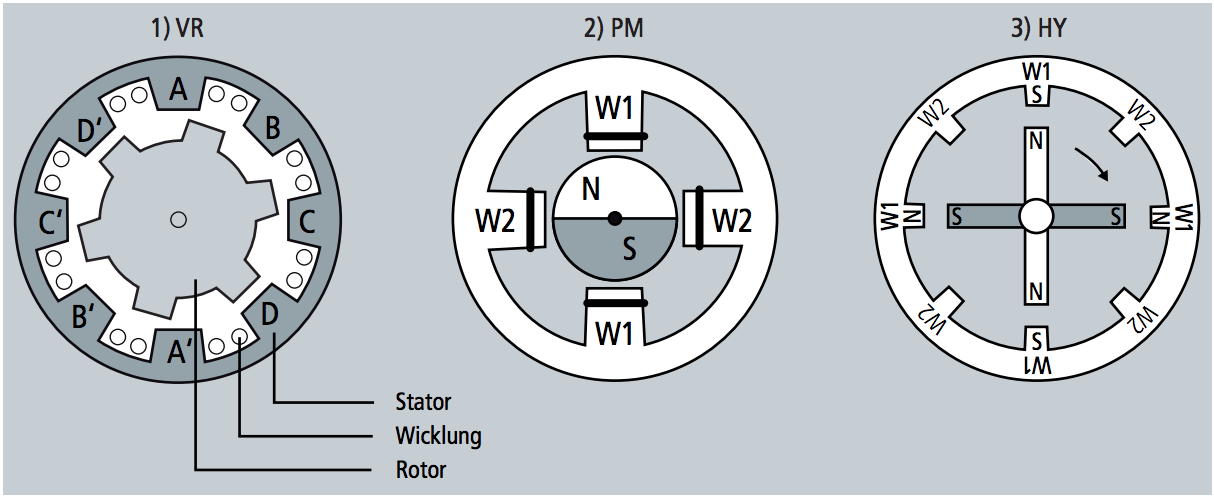
\includegraphics[width=1.0\textwidth]{images/Schrittmotortypen.png}
\caption{Schrittmotortypen \newline (Quelle: \cite{roboterKS_Bild})}
\label{robotKSys}
\end{figure}

Für unseren Anwendungsfall kommt nur der Hybridschrittmotor in Frage, aufgrund des Haltemomentes von 03 bis 1000 cNm und des kleinen Schrittwinkel von $0,36^\circ$.

\subsubsubsection{Hybridschrittmotor}
Der Hybridschrittmotor vereint die positiven Eigenschaften des Reluktanzschrittmotor und des Permanenterregten Schrittmotor. Sein Rotor besteht aus einem axialen Permanentmagneten, an dessen Enden gezahnte Kappen befestigt sind. Beide sind um eine halbe Zahnbreite gegeneinander versetzt, so das sich Nord- und Südpole abwechseln.

\subsubsubsection{Arten der Ansteuerung}
Es gibt drei Möglichkeiten Schrittmotoren anzusteuern.
\begin{itemize}
	\item Vollschritt
	\item Halbschritt
	\item Mikroschritt
\end{itemize}

In unserem Fall wird der Mikroschrittbetrieb benötigt um ein genaues Positionieren zu ermöglichen.
\subsubsubsection{Mikroschritt Betrieb}

\begin{quote}

Ein Schrittmotor führt Mikroschritte aus, wenn man die durch die Phasen fließenden Ströme nicht nur ein- oder ausschaltet, sondern in definierter Weise anwachsen und abnehmen läßt. Die Genauigkeit des Mikroschritts hängt davon ab, wieviele verschiedene Stromstärken vorgesehen sind und wie genau diese eingehalten werden. Die Theorie zeigt, daß eine sinusförmige Erregung am zweckmäßigsten ist. Es handelt sich dann eher um ein kontinuierliches Weiterdrehen als um ein ruckweises weiterschalten. Diese Betriebsweise hat einige Vorteile:
\begin{itemize}
	\item ruhigerer Lauf
	\item keine Resonanzeffekte
	\item Geräuschminderung
	\item Schonung der Lager und ggf. nachgeordneter Antriebsteile
	\item bessere Auflösung bzw. Positioniergenauigkeit
\end{itemize}

Die sinuförmige Erregung erreicht man durch Stromsteuerung, genauer durch Beeinflussung der Referenzspannung. Für jede Wicklung wird eine Referenzspannung gebildet, deren Zeitverlauf aufeinanderfolgenden Sinushalbwellen  entspricht. Beide Referenzspannungen sind gegeneinander um 90° phasenverschoben.

\end{quote}

\newpage

% !TEX root = ../SegwayDoku.tex
\renewcommand{\autoren}{Timo Veit}
\newpage
\subsection{Regelung von Schrittmotoren}
Da das Verwenden eines Schrittmotors zur Debatte stand, wurde hierzu eine Recherche angestellt.
Die Unterschiede zwischen einem BLDC-Motor und einem Schrittmotor sind im wesentlichen:
\par\bigskip

BLDC-Motor
\par\bigskip
\begin{tabularx}{\textwidth} {@{\hspace{1cm}}lX@{}}
    Verwendung von Drehstrom / 3 Phasen \\
    niedrige Polpaarzahl \\
\end{tabularx}

Schrittmotor
\par\bigskip
\begin{tabularx}{\textwidth} {@{\hspace{1cm}}lX@{}}
    meist Verwendung von 2 Phasen \\
    hohe Polpaarzahl \\
\end{tabularx}

\subsubsection{Auftrettende Schwierigkeiten}
Zur feldorienierten Vektorregelung bei BLDC Motoren wurden einige Erklärungen und die zugehörigen Berechnungen gefunden. Bei Schrittmotoren wird üblicherweise der Winkel geregelt, zur genauen Realisierung wird das sogenannte Microstepping verwendet. Dabei entstehen aber schwankende Momente. Eine Vorgehensweise um die Vektorregelung beim Schrittmotor mit 2 Phasen umzusetzen wurde nicht gefunden, ist aber grundsätzlich möglich.
Ein weiteres Problem ergibt sich aus der hohen Polpaarzahl. Bei 50 Polpaaren und einer einigermaßen guten Nachbildung des elektrischen Winkels mit 50 Stützstellen ergibt sich eine notwendige Decoderauflösung von 2500 Impulsen pro Umdrehung. Entsprechende Decoder sind wiederum teurer, dies macht den Preisvorteil des kostengünstigeren Schrittmotors zu nichte.
Die notwendige, hohe Auflösung führt ebenfalls dazu, dass zur Steuerung schon bei geringen Drehzahlen sehr hohe Frequenzen gebraucht werden.

\par\bigskip
\begin{tabularx}{\textwidth} {@{\hspace{1cm}}lX@{}}
	Pole p = 50 \\
	Stützstellen s = 50 \\
    U = 500 U/min \\
    Frequenz am Decoder: \\
    f = U / 60 * p * s = 20,8 kHz \\
\end{tabularx}

\subsubsection{Fazit}
Die Regelung des BLDC Motors ist einfacher Umzusetzen und der geringere Preis des Schrittmotors wird durch die teureren Decoder wieder marginalisiert.


\newpage

% !TEX root = ../SegwayDoku.tex
\renewcommand{\autoren}{Stephan Morongowski}
\newpage
\subsection{Auswahl der Motoren}

Grundsätzlich soll der Roboter mit einem Synchronmotor mit feldorientierter Regelung angetrieben werden, um diesen per Solldrehmoment regeln zu können.

In Abhängigkeit des verfügbaren Stromes von \(100 A\) (begrenzt durch den Motortreiber, siehe Abschnitt \ref{sssec:odrive}) ergibt sich für das gewünschte Spitzenmoment von ca. \(1 Nm\) eine Mindestdrehmomentkonstante von \(k_d \approx 0,01 \frac{Nm}{A}\) bzw. eine Drehzahlkonstante von \(k_v \approx  820 \frac{rpm}{V}\). Die Untergrenze für die Drehzahlkonstante ergibt sich aus der Maximalgeschwindigkeit des Roboters von \(5 \frac{km}{h}\) und damit ca. \(330 \frac{U}{min}\) zu ca. \(15 \frac{rpm}{V}\) bei \(U_{bat} = 22,2 V\). Dabei darf die maximal erlaubte Spannung des Motors \(22,2 V\) nicht überschreiten, um mit der verfügbaren Batteriespannung das maximale Moment auch erreichen zu können. Um eine möglichst kleine Baugröße zu erhalten, wurde vornehmlich nach Außenläufern gesucht, da bei dieser Bauform das mögliche Moment grundsätzlich größer ist, als bei Innenläufern.

Eine Liste der in Frage kommenden Motoren ist in Anhang ... beigefügt.

\label{sssec:RoxxyMotor}
Ausgewählt wurde der \glqq Roxxy BL Outrunner C50-55-45\grqq{}. Bei einem mittleren Preis bietet dieser Motor ein sehr hohes Moment von ca. \(1,5 Nm\) bei einer Nennspannung von nur \(12 V\) sowie einem ebenfalls geringen Spitzenstrom von \(16 A\). Damit werden alle Anforderungen erfült. Des Weiteren entstehen Vorteile wie geringere Kabelquerschnitte bei der Stromzuführung und geringere thermische Belastung des Motortreibers.
\newpage

% !TEX root = ../SegwayDoku.tex
\renewcommand{\autoren}{Stephan Morongowski}
\newpage
\subsection{Eigenbau eines Motortreibers}
Aufgrund der schlechten Verfügbarkeit eines zur feldorientierten Regelung von Synchronmotoren geeigneten Motortreibers wurde überlegt, einen solchen Treiber innerhalb der Projektarbeit zu entwickeln und zu bauen. Zur Eruierung des zeitlichen und kostenmäßigen Aufwandes wurden zunächst grobe Anforderungen festeglegt und anschließend eine Marktrecherche sowie eine Machbarkeitsstudie durchgeführt.

\subsubsection{Anforderungen an den zu entwickelnden Treiber}
Eine Skizze zur prinzipiellen Anordnung der nötigen Komponenten ist in Abbildung \ref{kompVec} gegeben.

\begin{figure}[h]  % [h] bedeutet, dass das Bild genau an dieser Stelle im Text erscheint
\centering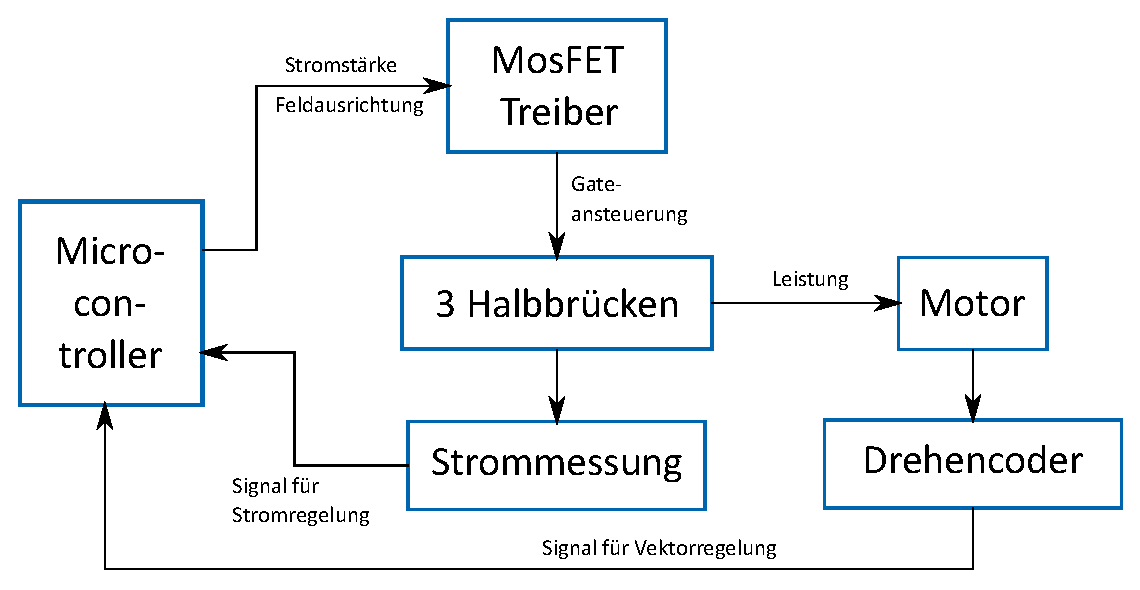
\includegraphics[width=0.8\textwidth]{images/KomponentenVektorregelung.eps}
\caption{notwendige Komponenten eines potentiellen Motortreibers \newline (Quelle: eigene Darstellung, SM)}
\label{kompVec}
\end{figure}

\begin{benannteAuflistung}[Notwendige Komponenten für zwei Motoren:]
    Microcontroller & 12-24 Pwm-Ausgänge pro Motor bei min. 20kHz \\
    & 4-6 digitale Eingänge für Quadraturencoder \\
    & 4 digitale Eingänge für Sollmomentvorgabe (Moment und Richtung) \\
    & 4 analoge Eingänge für Strommessung pro Motor \\
    Leisungstransistoren & 6 Halbbrücken (High-Side-Ansteuerung über Ladepumpe oder Pull-Up Widerstand zur Motorversorgungsspanung)  \\
    Sensorik & 4 mal Strommessung \\
\end{benannteAuflistung}

\par\bigskip

\begin{benannteAuflistung}[Gewünschte Technische Daten:]
    Motorspannung & bis 25V \\
    Strom & dauerhaft 30A, Spitze 50A \\
    Schnittstellen & I2C, USB, PWM \\
\end{benannteAuflistung}

\par\bigskip

Die Herstellungskosten sollten XXX,- € nicht übersteigen.

\par\bigskip



\subsubsection{Marktanalyse}

\subsubsubsection{VESC}
\label{sssec:vesc}
Der VESC - vector electronic speed control \cite{vesc} ist ein openSource Projekt von Benjamin Vedder. Der Treiber wurde ausgelegt, um ein Skateboard mit einem bürstenlosen Gleichstrommotor anzutreiben und ist in der Lage, 240A Spitzenstrom und 50A Dauerstrom bei bis zu 60V Versorgungsspannung zu liefern. Er verfügt über eine umfangreiche Konfigurationssoftware, über die vom PC aus alle nötigen Voreinstellungen vorgenommen werden können. Das ganze Projekt wirkt auf den ersten Eindruck sehr ausgereift.


\par\bigskip
\begin{benannteAuflistung}[Technische Daten:]
    Microcontroller & STM34F4 \\
    MOSFET Treiber & DRV8302 \\
    MOSFETS & 6 IRFS7530 \\
    Motorspannung & 8V - 60V \\
    Strom & dauerhaft 50A, Spitze 240A \\
    Schnittstellen & PPM signal (RC servo), analog, UART, I2C, USB, CAN-Bus \\
    Größe & 40mm mal 60mm \\
\end{benannteAuflistung}

\par\bigskip


\begin{benannteAuflistung}[Kosten im Eigenbau für zwei Stück:]
    Bauteile & ca. 120,- € \\
    Platinen & ca. 100,- €\\
    Lötzubehör & ca. 20,- € \\
    \textbf{Summe} & \textbf{ca. 240,- €} \\
\end{benannteAuflistung}

\par\bigskip
Beschaffungskosten für zwei fertig aufgebaute Platinen: \textbf{ca. 280,-€}

\newpage
\subsubsubsection{ODrive}
\label{sssec:odrive}
Der ODrive ist eine Entwicklung verschiedener Personen, da grundsätzlich jeder an der Entwicklung des Treibers teilnehmen kann. Dieser Treiber steuert bis zu zwei Motoren mit je ca. 100A Spitzenstrom. Das Projekt befindet sich noch in der Entwicklungsphase. Die Konfiguration des Treibers muss in die Firmware kompiliert werden.

\par\bigskip




\par\bigskip
\begin{benannteAuflistung}[Technische Daten:]
    Microcontroller & STM34F4 \\
    MOSFET Treiber & DRV8301 \\
    MOSFETS & 28 NTMFS4935NT1G \\
    Motorspannung & 8V - 30V \\
    Strom & dauerhaft ?, Spitze > 100A \\
    Schnittstellen & USB, CAN, UART, PWM, and step/dir interface \\
    Größe & 110mm mal 50mm \\
\end{benannteAuflistung}


\par\bigskip



\begin{benannteAuflistung}[Kosten im Eigenbau pro Stück:]
    Bauteile & ca. ???,- € \\
    Platinen & ca. ???,- €\\
    Lötzubehör & ca. 20,- € \\
    \textbf{Summe} & \textbf{ca. ???,- €} \\
\end{benannteAuflistung}

\par\bigskip
Beschaffungskosten als fertig aufgebaute Platine: \textbf{ca. 120,-€}

\subsubsubsection{Predriver}
Zur effizienteren Nutzung der MosFET wird von verschiedenen Herstellern ein Predriver angeboten. Zur Verfügung steht z.B. der DRV8305 von TI. Er stellt als Funktionen die nötige Ladepumpe, eine Möglichkeit zur Strommessung, optimierte Schaltung der FETs und andere Funktionen zur Verfügung.

\subsubsubsection{fertige Halbbrücke als Smd-Bauteil}
Infineon hat fertige Halbbrücken im Programm, die einige der benötigten Anforderungen bereits ohne externe Komponenten erfüllen. Als Beispiel sei hier der BTN8962TA vorgestellt:

\par\bigskip
\begin{benannteAuflistung}[BTN8962TA]
    Strom & dauerhaft 30A, Spitze 70A \\
    Spannung & bis 40V \\
	Ladepumpe & integriert \\
	Strommessung & integriert \\
	PWM & bis 25kHz \\
	Ansteuerung & logic level \\
	benötigte Menge & 6 Stück \\
	Einzelpreis & ca. 4,22€ \\
	\textbf{Gesamtkosten} & \textbf{ca. 25,-€} \\
\end{benannteAuflistung}

\subsubsubsection{Aufbau der Halbbrücken aus Einzelkompoenten}
\begin{benannteAuflistung}[Benötigte Komponenten][llX]
    MosFETs & 6 n-FETs  & ca. 3,-€ \\
	& 6 p-FETs & ca. 3,-€ \\
	Predriver & zB & ca. 5,-€ \\
	Strommessung & 4 Shuntwiderstände & ca. 3,-€ \\
	\textbf{Gesamtkosten} & & \textbf{ca. 14,-€} \\
\end{benannteAuflistung}

\subsubsubsection{Auswahl eines Microcontrollers}
\begin{benannteAuflistung}[Benötigte Eigenschaften pro Motor]
    6 Pwm-Ausgänge pro Motor bei min. 20kHz \\
    6 digitale Ausgänge pro Motor \\
    2-3 digitale Eingänge für Quadraturencoder \\
    2 digitale Eingänge für Sollmomentvorgabe (Moment und Richtung) \\
    2 analoge Eingänge für Strommessung pro Motor \\
\end{benannteAuflistung}
\par\bigskip

Zusätzlich zu den o.g. Angaben muss der Controller gut programmierbar sein und sollte keine, für die Projekt- und Labormitarbeiter völlig neuartige, Programmierumgebung darstellen. Auf Grund dieser Vorgabe wird die Auswahl eingeschränkt auf Controller, die entweder von dem Arduino-Framework oder dem mbed-Framework unterstützt werden. 
\par \smallskip
\begin{benannteAuflistung}[mögliche Kanditaten]
    Atmega 1280 & ca. 9,-€ \\
    Atmega 2560 & ca. 10,-€ \\
    STM32F4 & ca. 9,-€ \\
    STM32F7 & ca. 10,-€ \\
\end{benannteAuflistung}
\par\smallskip
Die Controller von Atmel liegen bei gleichem Preis in ihrer Leistung deutlich unter der Leistung der Controller von ST.

\subsubsubsection{Komplettlösungen als integrierter Schaltkreis}
Auf dem Markt finden sich verschiedene Ein-Chip-Lösungen für den Betrieb eines Synchronmotors. Jedoch sind diese in der Regel für sensorlosen Antrieb ausgelegt und damit im Stillstand nicht gut betreibbar. Des Weiteren liegen die erreichbaren Ströme weit unter den Projektanforderungen.

\subsubsection{Fazit}
Der Ankauf fertiger Motortreiber ist zu teuer. Ein eigenständiger Nachbau der Controller Vesc (siehe \ref{sssec:vesc}) oder ODrive (siehe \ref{sssec:odrive}) wird in etwa die gleichen Kosten produzieren, wie die Anschaffung der fertig bestückten Platinen und zusätzliche Arbeit schaffen.
Andere fertige Lösungen stehen derzeit nicht zur Verfügung.\\
 Es erscheint demnach am Sinnvollsten, einen an die Projektanforderungen angepassten Controller im Eigenbau neu zu entwerfen.


\newpage

\newpage

% !TEX root = SegwayDoku.tex
\renewcommand{\autoren}{Stephan Morongowski}
\newpage
\section{Navigation}
\subsection{Sensorik}
Zur Verfügung stehen folgende Sensoren:
\begin{itemize}
\item Gyros in allen drei Raumachsen
\item Beschleunigungssensoren in allen drei Raumachsen
\item Inkrementalgeber der Räder
\item Ultraschallsensoren
\end{itemize}

\subsection{Bestimmung der Position im Welt-KS}

\subsubsection{Drehung um den Momentanpol}
\label{turningVelocityPole}
Zur Bestimmung der Position des Roboters in einem festen Koordinatensystem können die Inkrementalgeber der Antriebsmotoren benutzt werden.

\begin{figure}[h]  % [h] bedeutet, dass das Bild genau an dieser Stelle im Text erscheint
\centering\includegraphics[width=0.8\textwidth]{images/Kurvenkinematic.eps}
\caption{Rotation um den Momentanpol \newline (Quelle: eigene Darstellung, SM)}
\label{kurvenkinematik}
\end{figure}

Zur Ermittlung der aktuellen Position ist in Abbildung \ref{kurvenkinematik} die Kinematik einer Kurvenfahrt dargestellt, betrachtet für einen gedanklich sehr kleinen Zeitabschnitt. In diesem wird angenommen, dass die Geschwindigkeiten \(v_1\) und \(v_2\) beider Räder konstant bleiben. Dies sorgt für die Vereinfachung, dass der Roboter sich auf einer Kreisbahn um einen für die betrachtete Zeitspanne konstanten Momentanpol bewegt. Im Folgenden sind die durch den Inkrementalgeber erfassten Bogenlängen mit arc bezeichnet.
Es gilt:
\begin{flalign}
    % durch das & Zeichen werden alle Gleichungen an diesem Punkt ausgerichtet
	arc_{Rl} &  = \Delta\gamma\cdot r_{Rl}
	\label{eq:bogenmaß_1} \\
	arc_{Rr} & = \Delta\gamma\cdot r_{Rr}
	\label{eq:bogenmaß_2} \\
	r_{Rr} & = r_{Rl}  + l_a
	\label{eq:achsZuMomentanpol} \\
	\Delta arcs & = arc_{Rr} - arc_{Rl}
	\label{eq:arcsDef} \\
    r_S & = r_{Rr} - \frac{1}{2} l_a
	\label{eq:r_s}
\end{flalign}

Aus \eqref{eq:bogenmaß_1}, \eqref{eq:bogenmaß_2}, \eqref{eq:achsZuMomentanpol}, \eqref{eq:arcsDef} und \eqref{eq:r_s} folgen:
% hier keine Leerzeile machen, sonst wird der Abstand ganz groß
\begin{flalign}
    \Delta\gamma & = \frac{\Delta arcs}{l_a}
	\label{eq:deltaPhi} \\
    r_S & = \frac{arc_{Rr}}{\Delta\gamma} - \frac{1}{2} l_a =
    l_a\left(\frac{arc_{Rr}}{\Delta arcs}-\frac{1}{2}\right)
\end{flalign}

Timo Veit:
Die Verschiebungen aus den Geschwindigkeiten nenne ich erstmal $x_*$.
%In Simulink verwende ich erstmal die Geschwindigkeiten und integriere dann danach, um auf die richtige Einheit zu kommen. Da aus Geschwindigkeit mal Zeit wieder Strecke wird funktioniert das auch.

\begin{flalign}
	x_S &= \frac{x_2-x_1}{2}+x_1	\\
	r_S &=  \frac{l_a}{ \frac{x_2}{x_1}-1} +  \frac{l_a}{2}\\
	\Delta\gamma &= atan( \frac{x_S}{r_S})	
\end{flalign}
Durch Aufsummieren von \(\Delta\gamma\) nach jeder Auswertung der Inkrementalgeber kann somit ein ungefährer Absolutwinkel der Roboterachse zu einem festen KS berechnet werden.
\par\bigskip
Zur Bestimmung des Schwerpunktes in xy-Koordinaten wird die Verschiebung von
\(S_0\) zu \(S_1\) mit trigonometrischen Funktionen berechnet und anschließend aufsummiert. Es gilt:
\begin{flalign}
	\vec{S_1} = \vec{S_0} +
        \begin{pmatrix}
            -\sin{(\Delta \gamma)} \cdot r_S \cdot \sin{(\gamma_0)}
            - (r_S - \cos{(\Delta \gamma)} \cdot r_S) \cdot \cos{(\gamma_0}) \\
            \sin{(\Delta \gamma)} \cdot r_S \cdot \cos{(\gamma_0)}
            - (r_S - \cos{(\Delta \gamma)} \cdot r_S) \cdot \sin{(\gamma_0})
        \end{pmatrix}
	\label{eq:S_1}
\end{flalign}

bzw. vereinfacht:
\begin{flalign}
	\vec{S_1} = \vec{S_0} +
        \begin{pmatrix}
            r_S [\cos{(\gamma_0 + \Delta\gamma)} - \cos{\gamma_0}]  \\
            r_S [\sin{(\gamma_0 + \Delta\gamma)} - \sin{\gamma_0}]
        \end{pmatrix}
	\label{eq:S_1_easy}
\end{flalign}

\subsubsection{Vereinfachung}
\label{easyDeadReckoning}
Nachteilig an der in \ref{turningVelocityPole} beschriebenen Methode sind folgende zwei Punkte: Zum Einen muss eine Geradeausfahrt des Roboters als Spezialfall behandelt werden, da sonst eine Division durch Null erfolgen würde. Zum Zweiten finden die Berechnungen immer nahe einer Singularität statt. Für eine annähernde Geradeausfahrt wird $r_S$ sehr groß und $\Delta \gamma$ sehr klein, was zu großen Berechnungsfehlern führen kann.

Reagiert man nun auf jedes Pulssignal der Inkrementalgeber, wird eine der beiden Größen $arc_{Ri}$ zu Null und der Momentanpol liegt auf diesem Rad, welches sich annähernd nicht bewegt hat. So müssen nur vier Fälle bei der Summation der Lageänderungen beachtet werden:

\begin{itemize}
\item $R_l$ dreht sich vorwärts oder rückwärts
\item $R_r$ dreht sich vorwärts oder rückwärts
\end{itemize}

Für jeden dieser Fälle können nun die Positionsänderungen $\Delta\gamma$, $\Delta x$, $\Delta y$ im roboterfesten KS vorberechnet werden.
\begin{flalign}
    arc_{Rn} & = \frac{2\pi\cdot r_R}{n_{Enc}}  \\
	\Delta\gamma & = \frac{arc_{Rn}}{l_a}  \\
	\Delta x & = \frac{1}{2}l_a\sin{(\Delta\gamma)}  \\
	\Delta y & = \frac{1}{2}l_a ( \cos{(\Delta\gamma)} - 1) 
\end{flalign}
mit der Anzahl der Encoderimpulse pro Umdrehung $n_{Enc}$  \\ und dem Radius der Räder $r_R$. \\ \\
Bei jedem Impuls der Encoder werden nun in Abhängigkeit von $\gamma_0$ die vorberechneten Positionsänderungen mit Hilfe einer Drehmatrix in das Welt-KS transformiert und zu $S_0$ hinzuaddiert. Zu $\gamma_0$ wird jedes Mal nur der konstante Wert $\Delta\gamma$ addiert.
\begin{flalign}
    \prescript{0}{}{S_1} &= \prescript{0}{}{S_0} + \prescript{0}{}{T}_1  \prescript{1}{}{\vec{\Delta s}}
    = \prescript{0}{}{S_0} + 
        \begin{pmatrix}
            \cos{\gamma_0} & -\sin{\gamma_0}  \\
            \sin{\gamma_0} & \cos{\gamma_0}
        \end{pmatrix}
        \begin{pmatrix}
            \Delta x  \\
            \Delta y  
        \end{pmatrix} \\
    \gamma_1 &= \gamma_0 + \Delta\gamma
\end{flalign}

\subsubsection{Berücksichtigung des Kippwinkels}
Obiger Algorithmus setzt voraus, dass der Roboter aufrecht steht. Kippt der Roboter um seine y-Achse, werden alleine durch das Kippen die Encoder verdreht, was zu einer berechneten Positionsänderung führt, die gar nicht stattgefunden hat. Um dies zu kompensieren, reichen die Encoder als alleinige Information nicht aus. Da der Roboter einen Sensor zur Bestimmung des Kippwinkels besitzt, kann nun eine laufende Korrektur vorgenommen werden. Dabei ist zu beachten, dass der Fehler durch das Kippen auch von dem aktuellen Winkel $\gamma$ abhängig ist. Kippt der Roboter z.B. bei einem $\gamma$ von $0°$, entsteht ein Fehler in x-Richtung. Würde er sich nun auf der Stelle drehen auf ein $\gamma$ von $90\degree$ und der bei einem $\gamma$ von $0\degree$ entstandene Fehler weiterhin einfach abgezogen, würde die Position nun einen Ort mit einem Fehler in y-Richtung anzeigen. Deshalb wird bei jedem Encoderimpuls die Änderung des Kippwinkels im Vergleich zur letzten Encoderauswertung umgerechnet in einen Weg in x-Richtung des roboterfesten KS, anschließend in das Welt-KS transformiert und gleichzeitig mit der durch in Abschnitt \ref{easyDeadReckoning} falsch berechneten Welt-Position aufsummiert.

\begin{flalign}
    \prescript{0}{}{S_1} &= \prescript{0}{}{S_0} + \prescript{0}{}{T}_1  \prescript{1}{}{\vec{\Delta s}}
    = \prescript{0}{}{S_0} + 
        \begin{pmatrix}
            \cos{\gamma_0} & -\sin{\gamma_0}  \\
            \sin{\gamma_0} & \cos{\gamma_0}
        \end{pmatrix}
        \begin{pmatrix}
            \Delta x  \\
            \Delta y  
        \end{pmatrix} \\
    \gamma_1 &= \gamma_0 + \Delta\gamma
\end{flalign}


\newpage

% !TEX root = SegwayDoku.tex
\renewcommand{\autoren}{Timo Veit}
\newpage
\section{Physikalischer Zusammenhang zwischen Geschwindigkeit und Radius}

\begin{figure}[h]  % [h] bedeutet, dass das Bild genau an dieser Stelle im Text erscheint
\centering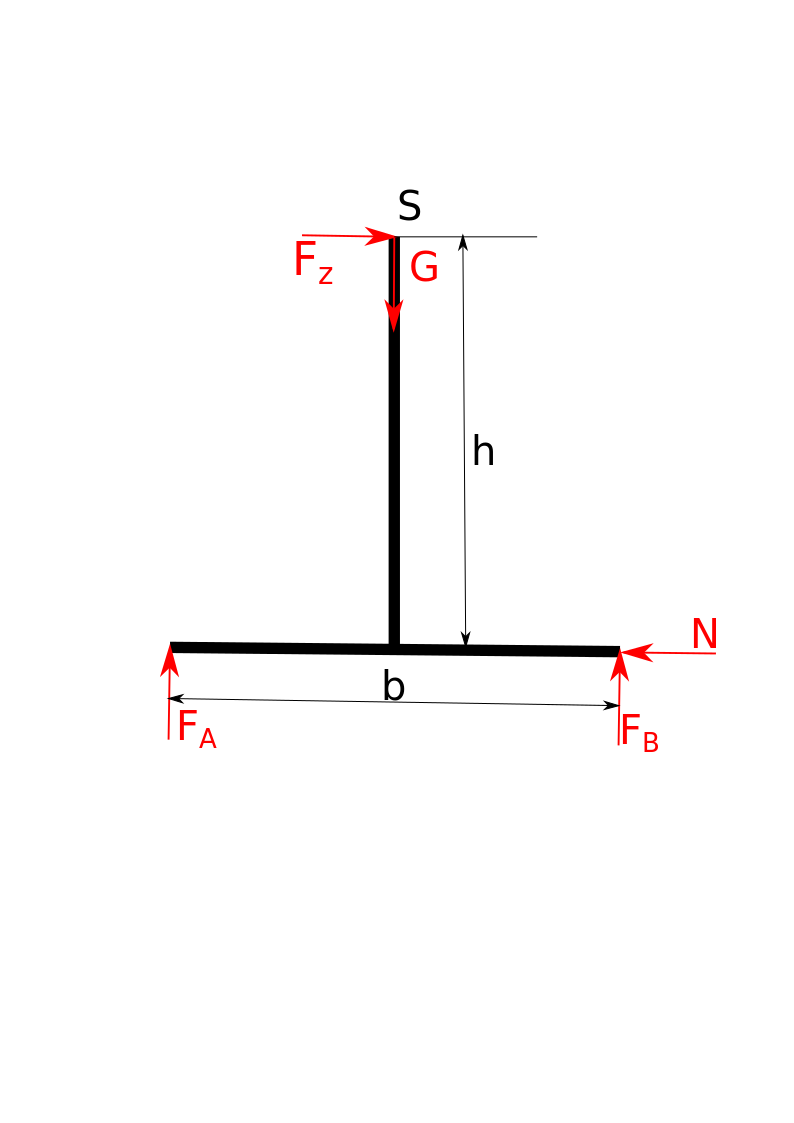
\includegraphics[width=0.6\textwidth]{images/SegwayFliehkraft.png}
\caption{Kräfte bei der Kurvenfahrt \newline}
\label{zentripetal}
\end{figure}

Bei der Kurvenfahrt darf der Roboter nicht seitlich umkippen. Um dies zu gewährleisten, muss das Verhältnis zwischen Geschwindigkeit und Kurvenradius passen. Dazu soll der innere Reifen noch mindestens die Hälfte der Last aufnehmen wie im Stand also ein Viertel der Gewichtskraft.

Es gilt:
\begin{flalign}
    % durch das & Zeichen werden alle Gleichungen an diesem Punkt ausgerichtet
	F_A &  = \frac{1}{4} m \cdot g
	\label{eq:gewichtskraft_1} \\
	G &  = m \cdot g
	\label{eq:gewichtskraft_2} \\
	F_{z} & = m \cdot \ddot x
	\label{eq:zentrifugalkraft} \\
	N & = m \cdot \frac{v^{2}}{r}
	\label{eq:zentripetalkraft} \\
	F_{A} + F_{B} & = G
	\label{eq:vertikale} \\
	N & = F_{z}
	\label{eq:horizontale} \\
    F_A \cdot b & = F_z \cdot h
	\label{eq:moment}
\end{flalign}

Aus \eqref{eq:bogenmaß_1}, \eqref{eq:bogenmaß_2}, \eqref{eq:achsZuMomentanpol}, \eqref{eq:arcsDef} und \eqref{eq:r_s} folgen:
% hier keine Leerzeile machen, sonst wird der Abstand ganz groß
\begin{flalign}
    \ddot x & = \frac{v^{2}}{r}
	\label{eq:xpp} \\
    \frac{1}{4} m \cdot g \cdot b & = m \cdot \frac{v^{2}}{r} \cdot h
	\label{eq:lsg_1} \\
\end{flalign}

Und daraus die Zusammenhänge von Geschwindigkeit zu Radius
\begin{flalign}
    v & = \sqrt{\dfrac{gb}{4h} \cdot r}
	\label{eq:lsg_v} \\
    r & = \dfrac{4h}{gb} \cdot v^2
	\label{eq:lsg_r} \\
\end{flalign}

Der notwendige Reibwert \(\mu\) zwischen Reifen und Boden ergibt sich aus der Haftbedingung.

\begin{flalign}
    \mu \cdot mg & = m \cdot \frac{v^{2}}{r}
	\label{eq:mu_1} \\
    \mu & = \frac{v^{2}}{rg}
	\label{eq:mu_2} \\
\end{flalign}
% !TEX root = SegwayDoku.tex
\renewcommand{\autoren}{Valentyn Chepil}
\newpage
\section{Die Hinderniserkennung}
\subsection{Ultraschallsensor}
% \ref{bild_3} zuweisung auf Bild in Text.

\begin{figure}[!h]  % [h] bedeutet, dass das Bild genau an dieser Stelle im Text erscheint
	% mit width=... wird die Größe des Bildes in Prozent der Seitenbreite eingestellt
	\centering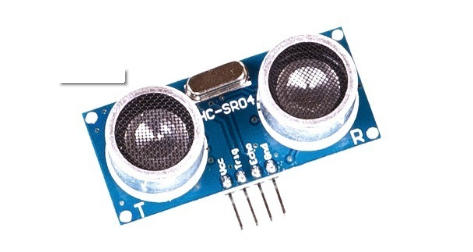
\includegraphics[width=0.5\textwidth]{images/Bild-1-1.png}
	% caption ist die Bildunterschrift, taucht auch im Abbildungsverzeichnis auf
	\caption{Ultraschallsensor \newline(Quelle: funduinoshop.com)}
	\label{bild_1.1} % über das label kann man aus dem Text auf das Bild verweisen
\end{figure}

\textbf{Parameter:}  %fett 
\begin{itemize} 
	\item Modul: HC-SR04 
	\item Preis:  1.50 Doller
\end{itemize}

Die Erkennung vom Hindernis erfolgt über ausgehenden Schallwellen, die sich in kegelförmig Form  ausbreiten. Bei Erreichung des Ziels werden die reflektierende Schallwellen aufgenommen und das Zeig des Reflektion wird ausgemessen. Dadurch erkennt man das Hindernis und den Abstand zu dem. Die Ausbreitung und die reflektierende Schallwellen hängt von verschiedenen Faktoren ab. Sie werden vom Luftdruck, der Umgebungstemperatur, der Luftfeuchtigkeit sowie vom Sende-/Empfangswinkel und der Oberfläche des im Schallkegel befindlichen Objekts
beeinflusst.

\begin{figure}[!h]  % [h] bedeutet, dass das Bild genau an dieser Stelle im Text erscheint
	\centering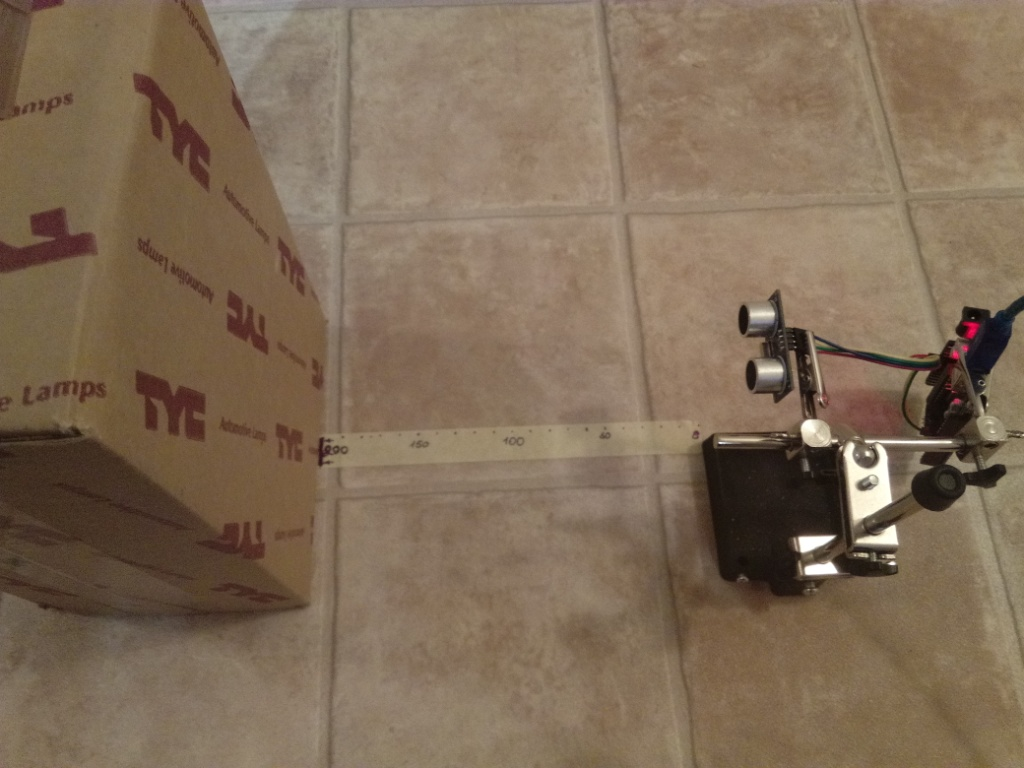
\includegraphics[width=0.6\textwidth]{images/Bild-1.jpg}
	\caption{Entfernungsmessung \newline (Quelle: eigene Darstellung, US-Sensor Messvorgang)}
	\label{bild_1} % über das label kann man aus dem Text auf das Bild verweisen
\end{figure}

\textbf{Vorteile:}  %fett 

Ein größter Vorteil des Ultraschallsensors ist günstiger Preis. Dies ermöglicht die Verwendung von vielen Sensoren bei der Modellbau, was zur präzisen Erfassung der Entfernung zu Hindernissen und Objekten in der Umgebung führt. Kann man in der Abbildung \ref{bild_1} sehen.

\par\bigskip %leere zeile
\textbf{Nachteile:}  %fett 

Ein Hindernis oder Objekt kann nicht genau geortet werden, sondern man kann nur feststellen, dass es sich in der gemessenen Entfernung innerhalb des Schallkegels befindet. Kann man in der Abbildung \ref{bild_2} sehen.

\begin{figure}[ht]  % [h] bedeutet, dass das Bild genau an dieser Stelle im Text erscheint
	\centering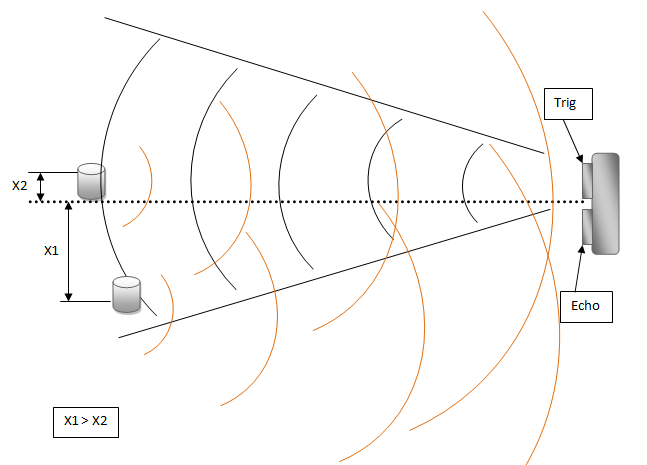
\includegraphics[width=0.6\textwidth]{images/Bild-2.png}
	\caption{Positionierung in Messbereich \newline (Quelle: eigene Darstellung)}
	\label{bild_2} % über das label kann man aus dem Text auf das Bild verweisen
\end{figure}

Bei mehrere Objekten vor Schallwelle wird der Abstand zum nächstliegenden Hindernis gemessen und die weit liegender Objekte werde einfach nicht erkannt. Kann man in der Abbildung \ref{bild_3} sehen.


\begin{figure}[ht]  % [h] bedeutet, dass das Bild genau an dieser Stelle im Text erscheint
	\centering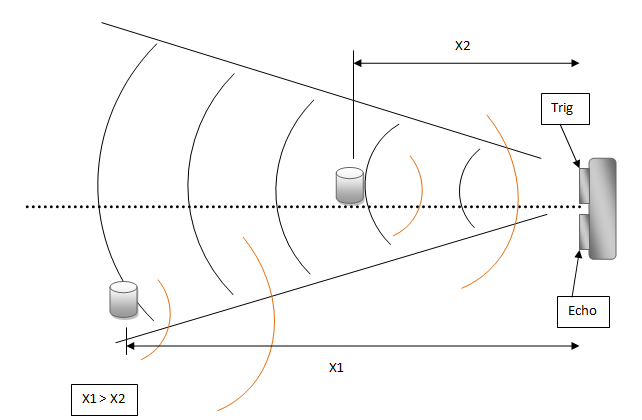
\includegraphics[width=0.6\textwidth]{images/Bild-3.png}
	\caption{Positionierung in Messbereich \newline (Quelle: eigene Darstellung)}
	\label{bild_3} % über das label kann man aus dem Text auf das Bild verweisen
\end{figure}

Als Nachteil kann man nennen die geringe Reichweite (ca. 3m) des Ultraschalls und  der geringen Ausbreitungsgeschwindigkeit des Schalls.

Große Probleme bekommt man auch aus den Reflektionseigenschaften der Schallwellen. Besonders bei weichen Materialien und spitzen-förmigen Oberflächen,
Oberflächenerkennung erfasst das Sensor auch schleicht. Das kann man in der Abbildung \ref{bild_4} sehen.

\begin{figure}[!h]  % [h] bedeutet, dass das Bild genau an dieser Stelle im Text erscheint
	\centering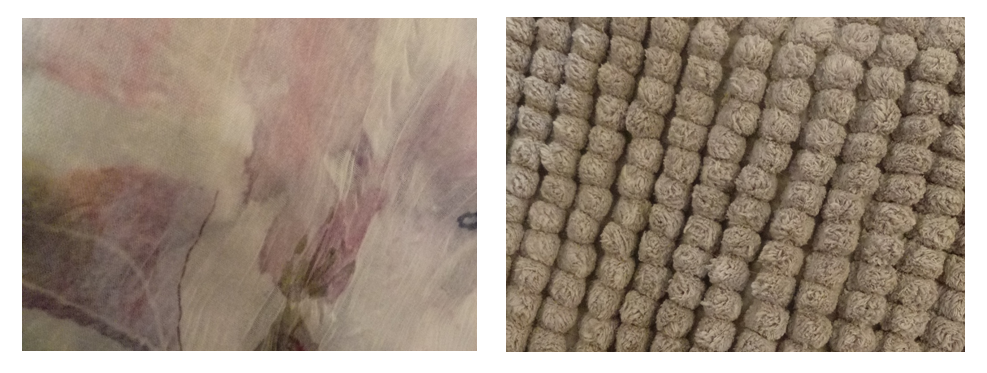
\includegraphics[width=0.8\textwidth]{images/Bild-4-5.png}
	\caption{Weiche und spitzen-förmige-weiche Oberflächen \newline(Quelle: eigene Darstellung,Frauen-Halsschal und Teppich)}
	\label{bild_4}
\end{figure}

\begin{figure}[!h]  % [h] bedeutet, dass das Bild genau an dieser Stelle im Text erscheint
	\centering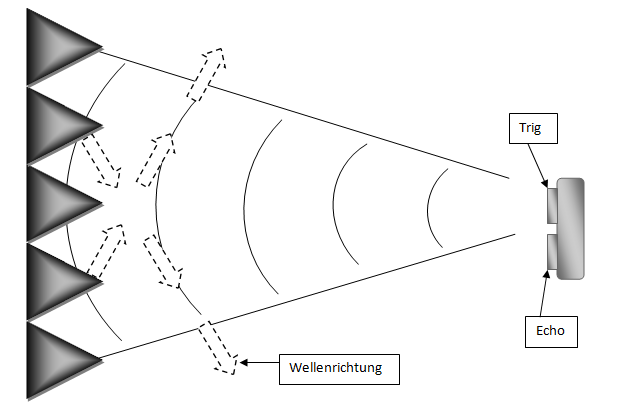
\includegraphics[width=0.55\textwidth]{images/Bild-6.png}
	\caption{Spitzen-förmige Oberflächen\newline(Quelle: eigene Darstellung, z.B: Kanten)}
	\label{bild_6}
\end{figure}

\begin{figure}[!h]  % [h] bedeutet, dass das Bild genau an dieser Stelle im Text erscheint
	\centering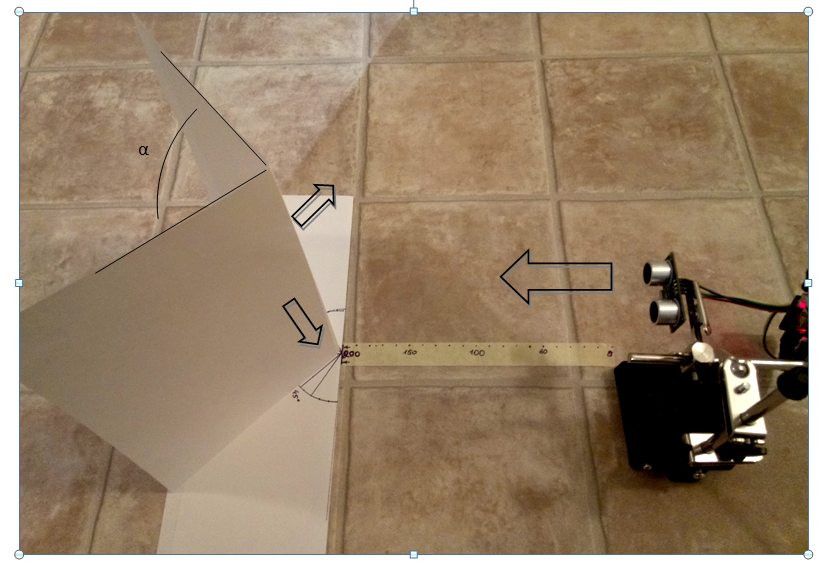
\includegraphics[width=0.5\textwidth]{images/Bild-7.png}
	\caption{Öffnungswinkel (Quelle: eigene Darstellung)}
	\label{bild_7} % über das label kann man aus dem Text auf das Bild verweisen
\end{figure}
Wird das Winkel des Schallkegels größer seinem Öffnungswinkel auf eine ebene Wand, so erreicht die Reflektion den aussendenden Sensor nicht. Kann man am Abbildung \ref{bild_7} sehen.





\subsection{Laser Sensor - Variante 1}
\begin{figure}[!h]  % [h] bedeutet, dass das Bild genau an dieser Stelle im Text erscheint
	\centering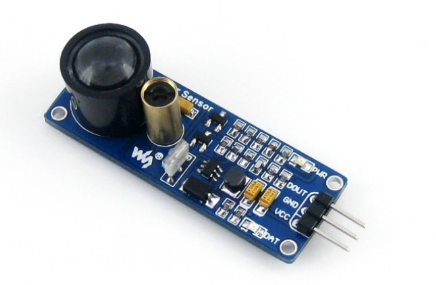
\includegraphics[width=0.6\textwidth]{images/laser-sensor.png}
	\caption{Laser-Sensor (Quelle: waveshare.com)}
	\label{laser-sensor} % über das label kann man aus dem Text auf das Bild verweisen
\end{figure}

\textbf{Parameter:}  %fett 
\begin{itemize}
\item Modul: 
\item Chip-Name: PT1301
\item Preis: 10.79 Doller
\item Quelle: https://www.waveshare.com/Laser-Sensor.htm
\end{itemize}
\begin{figure}[!h]  % [h] bedeutet, dass das Bild genau an dieser Stelle im Text erscheint
	\centering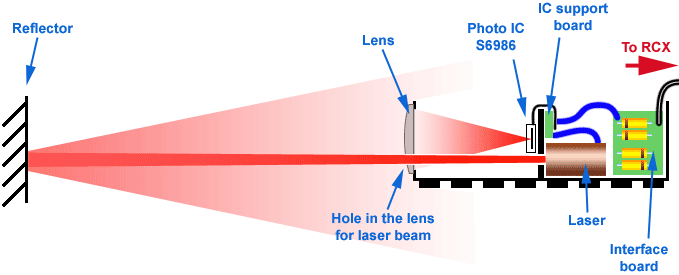
\includegraphics[width=0.9\textwidth]{images/laser-sensor1.png}
	\caption{ \ Aufbau der Sensors (Quelle:philohome.com)}
	\label{laser-sensor1} % über das label kann man aus dem Text auf das Bild verweisen
\end{figure}

\par\bigskip %leere zeile
\textbf{Vorteile:}  %fett 

\par\bigskip %leere zeile
\textbf{Nachteile:}  %fett 




\pagebreak

\subsection{Laser Sensor - Variante 2}
\begin{figure}[htbp!]  % [h] bedeutet, dass das Bild genau an dieser Stelle im Text erscheint
	\centering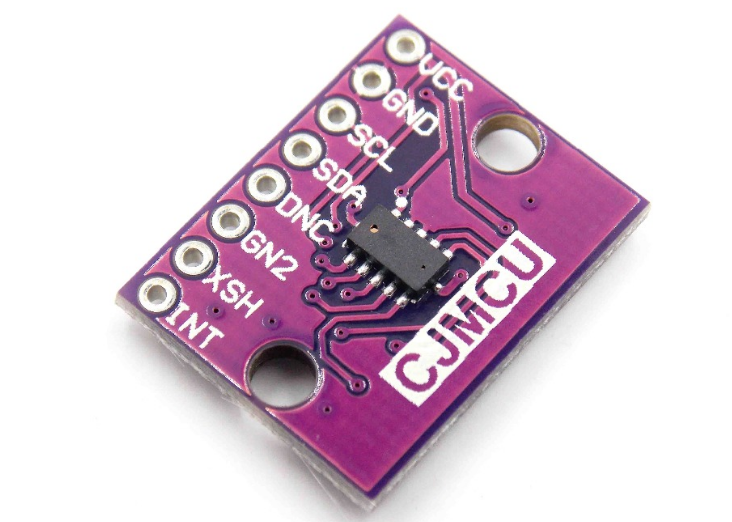
\includegraphics[width=0.6\textwidth]{images/laser-sensor_v2.png}
	\caption{ \ Laser-Sensor-VL53L0X (Quelle: ebay.de)}
	\label{laser-sensor_v2} % über das label kann man aus dem Text auf das Bild verweisen
\end{figure}

\textbf{Parameter:}  %fett 

\begin{itemize}
\item Modul: CJMCU-530
\item Chip-Name: VL53L0X
\item Preis: 4,84 Doller
\end{itemize}

\par\bigskip %leere zeile
\textbf{Vorteile:}  %fett 

\par\bigskip %leere zeile
\textbf{Nachteile:}  %fett 

\subsection{Infrarot Sensor}

\begin{figure}[ht]  % [h] bedeutet, dass das Bild genau an dieser Stelle im Text erscheint
	\centering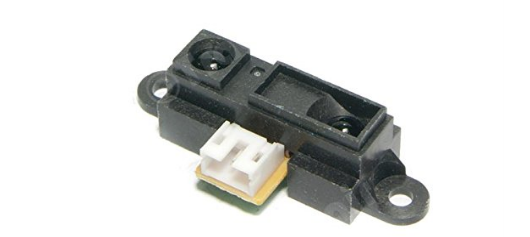
\includegraphics[width=0.8\textwidth]{images/infrarot.png}
	\caption{ \ Infrarot-Sensor  (Quelle: amazon.de)}
	\label{infrarot} % über das label kann man aus dem Text auf das Bild verweisen
\end{figure}

\textbf{Parameter:}  %fett 

\begin{itemize}
\item Modul: 
\item Preis: 1,53 Doller
\item Kommunikation: Analog Output Voltage (typischerweise 0,4 bis 2,3 V Range)
\item Betriebstemperatur:-10 bis + 60 °C
\item Minimale Messdistanz = 10 cm
\item Maximale Messdistanz = 80 cm
\item Reaktionszeit = 38 ± 10 ms
\end{itemize}

\par\bigskip %leere zeile
\textbf{Vorteile:}  %fett 

\par\bigskip %leere zeile
\textbf{Nachteile:}  %fett 

Datenblatt – > http://makertreeebayimages.azurewebsites.net/ebayimages/ebaycontent/gp2y0 a21yk-data-sheet.pdf 
Dieses Sensor sendet ein Strahl des Infrarot-Licht auf ein Objekt und wartet  reflektierte Licht zurück kommt.
% !TEX root = SegwayDoku.tex
\newpage
\renewcommand{\autoren}{Valentyn Chepil}
\section{Die Hindernis umfahren}

Die benötigten, reaktiven Fähigkeiten ”Hindernis umfahren”, (bzw. ”Hindernis rechts umfahren” und ”Hindernis links umfahren”) können alternativ mithilfe der Regelungstechnik und zweier grundlegender Teilschritte realisiert werden. Der prinzipielle Ablauf der reaktiven Fähigkeit ist in Abbildung \ref{bild_HUR} dargestellt. 

\begin{figure}[!h]  % [h] bedeutet, dass das Bild genau an dieser Stelle im Text erscheint
	\centering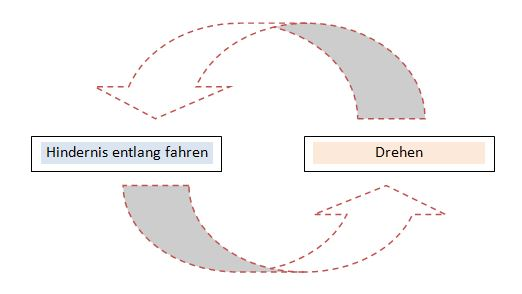
\includegraphics[width=0.6\textwidth]{images/Bild-HUR.jpg}
	\caption{ \ Regelkreis "Hindernis umfahren" (Quelle:Eigene Darstellung)}
	\label{bild_HUR} % über das label kann man aus dem Text auf das Bild verweisen
\end{figure}

In der Abbildung sind zwei prinzipielle Teilschritte abgebildet und durch zwei Farben gekennzeichnet. Zuerst soll sich der Glied in Bezug auf das Hindernis entscheiden, siehe Teilschritt ”Fallauswahl” - Bild \ref{baum2} , anschließend entlang des Hindernisses fahren. Diese beiden Teilschritte werden noch weiter unterteilt. Der Schritt Drehen wird je nach vorgegebener Richtung in ”Drehen rechts” und ”Drehen links” aufgeteilt. Dieser Teilschritt wird als vorgegebene Konstante realisiert und da als Winkel (0 Grad, positiv oder negativ) definiert. ”Hindernis entlang fahren” wird in die Teilschritte "Hindernis rechts entlang Fahren" und "Hindernis links entlang Fahren". Dieser Teilschritt wird als vorgegebene Konstante realisiert

\subsection{Ampelsysten}

Es wurde drei Zone (grün, gelb, rot) von mir definiert, die sich wie "Ampelsysten"  (Abbildung \ref{zone}) verhalten. Im grünen Bereich fährt den Roboter mit voller Geschwindigkeit \textcolor{green}{\textit{skal\_zone=1}}. Bei Erkennung des Hindernis in gelber Zone bremst dem Roboter langsam ab \textcolor{green}{\textit{skal\_zone=0.4}} und fängt manövrieren \textcolor{green}{\textit{drehwinkel=0 Grad, positiv oder negativ}}. Die Geschwindigkeit  des Roboters in roter Zone geht auf 0 \textcolor{green}{\textit{skal\_zone=0}}. Den Roboter im Stillstand sucht als weiterer Schritt einen freien Weg zum Ziel über Teilprogramm "Fallauswahl". In der Abbildung \ref{baum2} ist zu sehen.

Aus der Fähigkeiten des US-Sensors wurde folgende Entfernung in einzelner Zonen definiert:
\begin{figure}[!h]  % [h] bedeutet, dass das Bild genau an dieser Stelle im Text erscheint
	\centering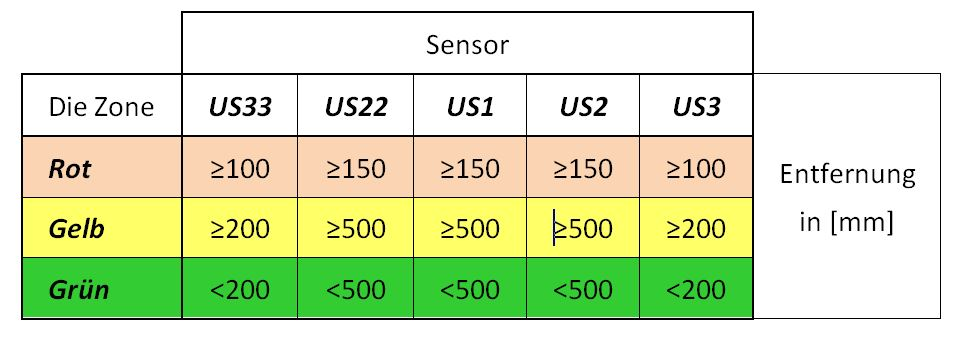
\includegraphics[width=0.60\textwidth]{images/entf.jpg}
	\label{entf} % über das label kann man aus dem Text auf das Bild verweisen
\end{figure}

\begin{figure}[!h]  % [h] bedeutet, dass das Bild genau an dieser Stelle im Text erscheint
	\centering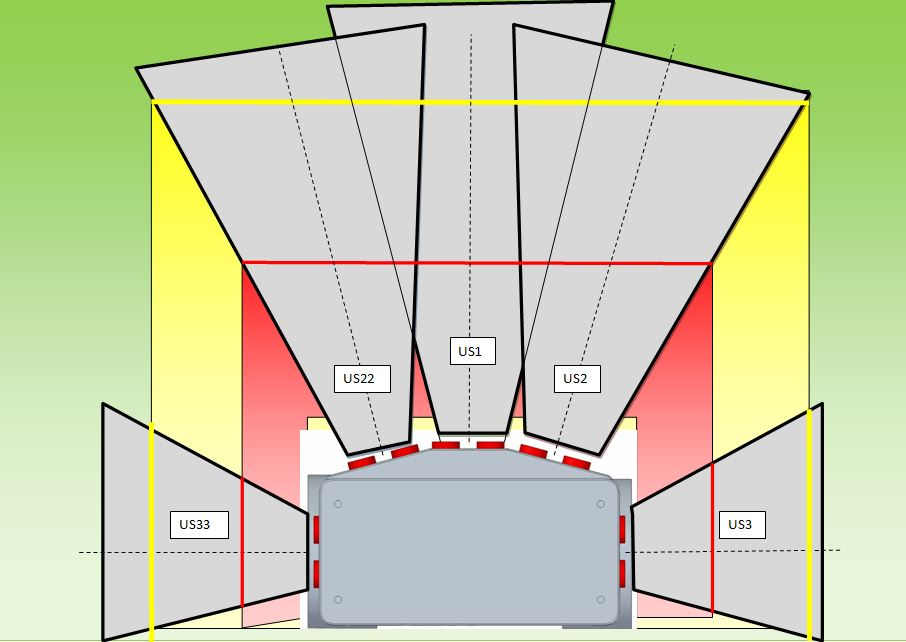
\includegraphics[width=0.85\textwidth]{images/H-UMF.jpg}
	\caption{ "Ampelsysten" zur Steuerung der Geschwindigkeit (Quelle:Eigene Darstellung)}
	\label{zone} % über das label kann man aus dem Text auf das Bild verweisen
\end{figure}

\subsection{Fallauswahl}

Es wurde unter sechs Fälle entschieden. Die alle Fälle sind auf Abbildung \ref{faelle} zu betrachten.

\begin{figure}[!h]  % [h] bedeutet, dass das Bild genau an dieser Stelle im Text erscheint
	\centering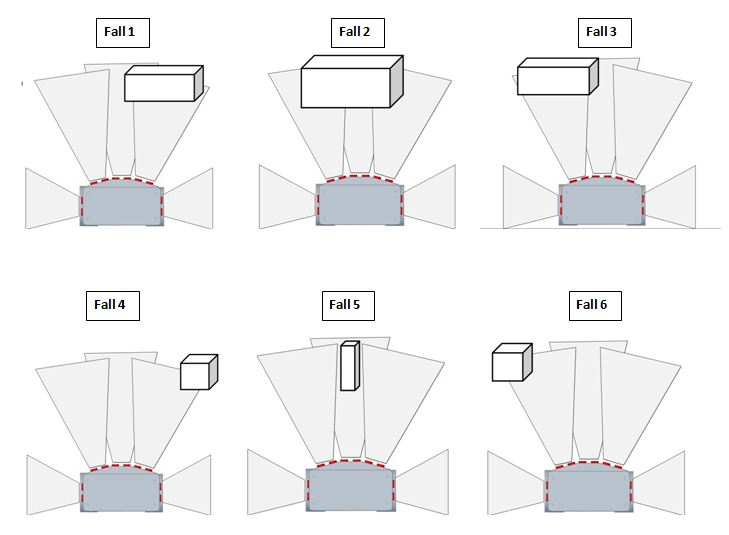
\includegraphics[width=0.7\textwidth]{images/faelle.jpg}
	\caption{ Entscheidungsmöglichkeiten (Quelle:Eigene Darstellung)}
	\label{faelle} % über das label kann man aus dem Text auf das Bild verweisen
\end{figure}

\subsection{Entscheidungsbaum}

 In diesem Fall wird in Abhängigkeit von der aktuellen Orientierung des Hindernis entschieden, wie es am günstigsten ist sich zu drehen, um das Fahren entlang des Hindernisses fortzusetzen. 
 
\begin{figure}[!h] 
	\centering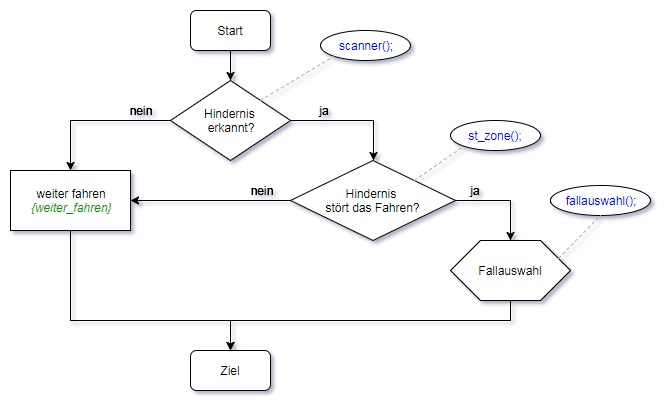
\includegraphics[width=0.75\textwidth]{images/Entsch-baum1.jpg}
	\caption{ \ Entscheidungsbaum für "Hindernis umfahren";\textcolor{blue}{\textit{scanner(); skal\_zone();}} und \textcolor{blue}{\textit {fallauswahl();}} sind Teilprogramme;   (Quelle:Eigene Darstellung)}
	\label{baum1} 
\end{figure}

Im Strukturgramm sieht man schön, wie der Roboter sich vor einem Hindernis verhalten soll. Um eine Prüfung des Hinderniserkennung zu starten muss man Zielkoordinaten eingeben. Danach fängt den Roboter scannen und die Ergebnisse zu bewerten. Für die Bewertung wurde hier wieder eine vereinfachte grafische Darstellung - Bild \ref{baum2} erstellt.

In nachfolgender Abbildung \ref{baum2} wird das Teilprogramm so lange aufgefordert ein Hindernis umzufahren, bis er nicht mehr stört.

\begin{figure}[!h]  % [h] bedeutet, dass das Bild genau an dieser Stelle im Text erscheint
	\centering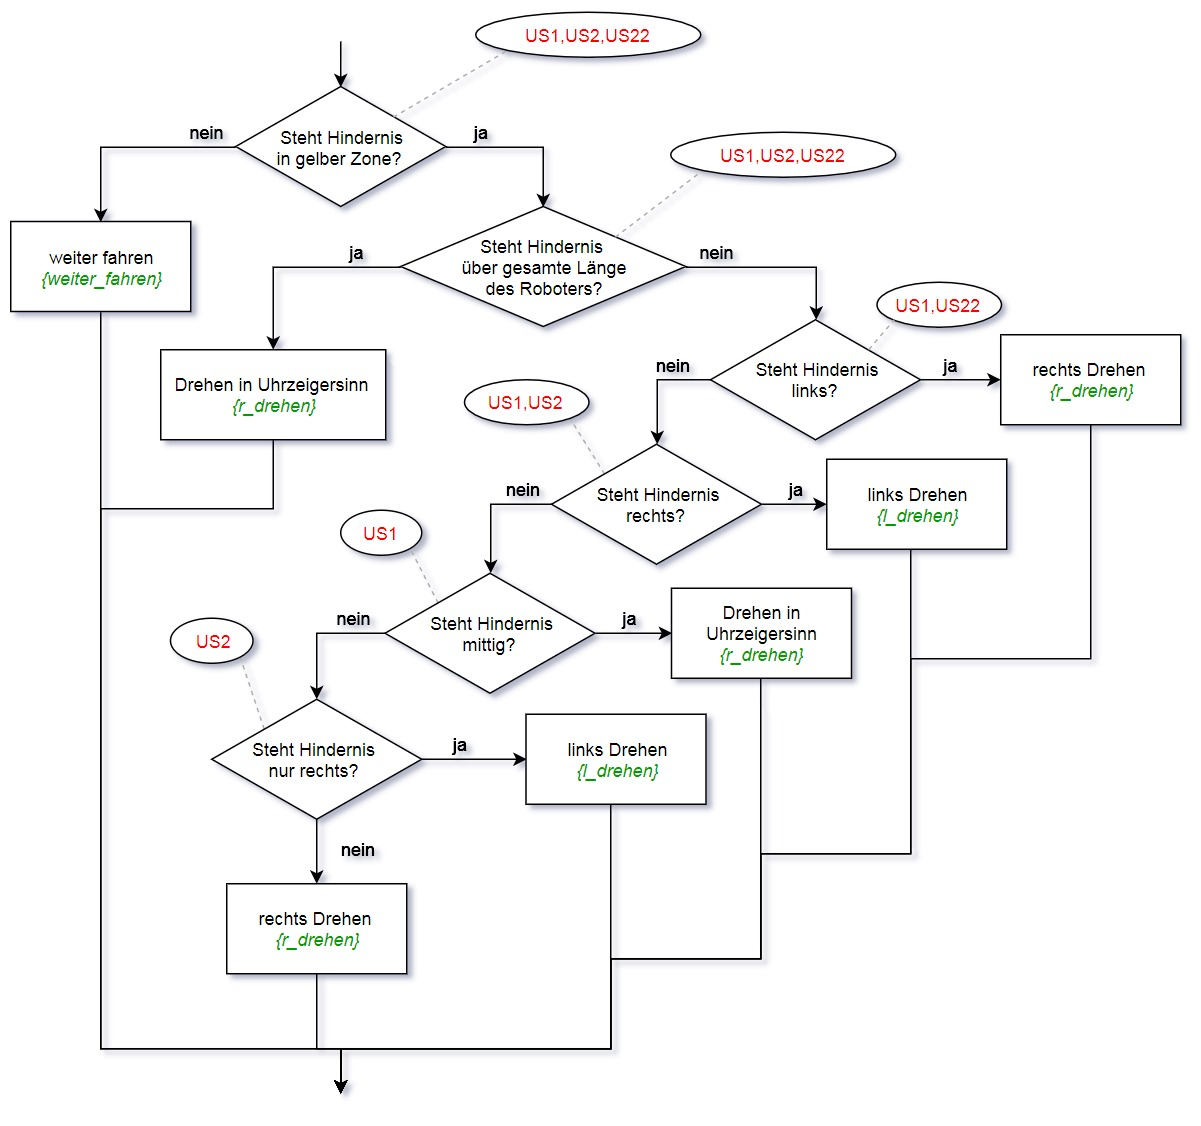
\includegraphics[width=0.99\textwidth]{images/Entsch-baum2.jpg}
	\caption{ Fallauswahl bei "Hindernis umfahren" (Quelle:Eigene Darstellung)}
	\label{baum2} % über das label kann man aus dem Text auf das Bild verweisen
\end{figure}
\pagebreak

\subsection{Arduino-Code}

Mit der Hilfe von Arduino-Uno senden man die Sensorwerte und Bewegungsverhalten an mBed-Platine. 

\begin{lstlisting}[language=C++, caption=Code zur Hinderniserkennung und Hindernif umfahren, label={lst:deadReackon}]
#include <NewPing.h>
#define Trig_Pin_33   6
#define Echo_Pin_33   7
#define Trig_Pin_22  12
#define Echo_Pin_22  13
#define Trig_Pin_1   8
#define Echo_Pin_1   9
#define Trig_Pin_2   10
#define Echo_Pin_2   11
#define Trig_Pin_3   4
#define Echo_Pin_3   5
#define Max_Distance 200

NewPing sonar1 (Trig_Pin_1, Echo_Pin_1, Max_Distance);
NewPing sonar2 (Trig_Pin_2, Echo_Pin_2, Max_Distance);
NewPing sonar22 (Trig_Pin_22, Echo_Pin_22, Max_Distance);
NewPing sonar3 (Trig_Pin_3, Echo_Pin_3, Max_Distance);
NewPing sonar33 (Trig_Pin_33, Echo_Pin_33, Max_Distance);

float skalierung;
float duration1;
float duration2;
float duration22;
float duration3;
float duration33;
float US1;                      //Sensor front middl
float US2;                      //Sensor front right
float US22;                     //Sensor front left
float US3;                      //Sensor side right
float US33;                     //Sensor side left
float soundsp;
float soundcm;
int interations = 3;

int skal_zone;            
//Skalierung zone = 1 sehr langsam / zone = 2 langsam / zone = 3 norm. fahren
int winkel;               
//bei winkel=1 färht er gerade aus./ winken=0 (minus Winkel) / winken=2 (plüs Winkel)

void sk_zone(void);
void langsam_fahren(void);
void fallauswahl(void);
void IBO_drehen(void);  
void go_drehen(void);
void l_drehen(void); 
void r_drehen(void);
void weiter_fahren(void);  
void langsam_fahren(void);   
void rueckwertsfahren(void);

void setup() {
Serial.begin(9600);
pinMode(Trig_Pin_1, OUTPUT);
pinMode(Echo_Pin_1, INPUT);
pinMode(Trig_Pin_2, OUTPUT);
pinMode(Echo_Pin_2, INPUT);
pinMode(Trig_Pin_22, OUTPUT);
pinMode(Echo_Pin_22, INPUT);
pinMode(Trig_Pin_3, OUTPUT);
pinMode(Echo_Pin_3, INPUT);
pinMode(Trig_Pin_33, OUTPUT);
pinMode(Echo_Pin_33, INPUT); }

void loop()    {
scanner();
sk_zone();
fallauswahl(); }

void scanner(){
duration1 = sonar1.ping_median(interations);
US1 = (duration1 / 2) * 0.0341;
duration2 = sonar2.ping_median(interations);
US2 = (duration2 / 2) * 0.0341;
duration22 = sonar22.ping_median(interations);
US22 = (duration22 / 2) * 0.0341;
duration3 = sonar3.ping_median(interations);
US3 = (duration3 / 2) * 0.0341;
duration33 = sonar33.ping_median(interations);  
US33 = (duration33 / 2) * 0.0341; }

void sk_zone() {  
//zone = 1 anhalten und drehen / zone = 2 langsam und abbiegen / zone = 3 norm. fahren

if ((US1 > 15 && US1 < 50)  || (US2 > 15 && US2 < 50)  || (US22 > 15 && US22 < 50) || (US3 > 10 && US3 < 30) || (US33 > 10 && US33 < 30)){
skal_zone = 1;  }
else if ((US1>2 && US1<15) || (US2>2 && US2<15) || (US22>2 && US22<15 ) || (US3>2 && US3<10) || (US33>2 && US33<10)){
skal_zone = 0;  }
else { skal_zone = 4; } }

void fallauswahl(){ 
if ((US1>2 && US1<15) || (US2>2 && US2<15) || (US22>2 && US22<15) || (US3>3 && US3<10) || (US33>3 && US33<10)) { langsam_fahren();
if ((US3>3 && US3<10) || (US33>3 && US33<10)) {
if (US3>2 && US3<10)   { l_drehen();  } 
else                   { r_drehen();  } } }
else if ( (US1>2 && US1<50) || (US2>2 && US2<50) || (US22>2 &&  US22<50)) 
{ langsam_fahren(); 
if ((US1>2 && US1<50) && (US2>2 && US2<50) && (US22>2 &&  US22<50)) 
{ go_drehen();  }
else if ((US1>2 && US1<50)  && ( US22>2 && US22<50))
{ r_drehen();   }
else if ((US1>2 && US1<50) && (US2>2 && US2<50))  { l_drehen();   }
else if (US1>2 && US1<50)                 { r_drehen();   }
else if (US2>2 && US2<50)                 { l_drehen();   }
else                                      { r_drehen();   } }
else                                      { weiter_fahren(); } }

void langsam_fahren(){   
winkel = 0;
Serial.write(skal_zone);
Serial.write(winkel);
Serial.println(); }

void weiter_fahren(){   
winkel = 0;
Serial.write(skal_zone);
Serial.write(winkel);
Serial.println(); }

void r_drehen(){ 
winkel = -2;
Serial.write(skal_zone);
Serial.write(winkel);
Serial.println(); }

void l_drehen(){ 
winkel = 2;
Serial.write(skal_zone);
Serial.write(winkel);
Serial.println(); }

\end{lstlisting}

\pagebreak
% !TEX root = SegwayDoku.tex
\newpage
\renewcommand{\autoren}{Valentyn Chepil}
\section{Die Gehäuse}
\subsection{Die Gehäusen - V.1}
% \ref{bild_3} zuweisung auf Bild in Text.
\begin{figure}[!h]  % [h] bedeutet, dass das Bild genau an dieser Stelle im Text erscheint
	% mit width=... wird die Größe des Bildes in Prozent der Seitenbreite eingestellt
	\centering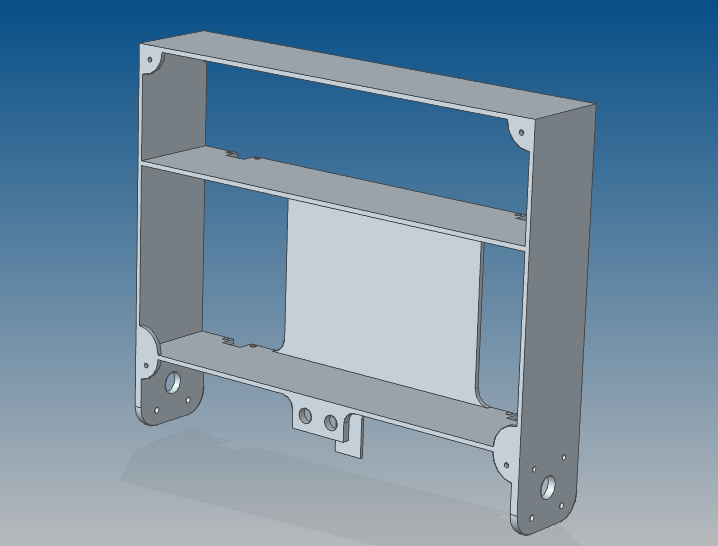
\includegraphics[width=0.5\textwidth]{images/gehaeuse-v1.png}
	% caption ist die Bildunterschrift, taucht auch im Abbildungsverzeichnis auf
	\caption{Gehäuse - V.1 \newline (Quelle: eigene Darstellung)}
	\label{gehaeuse-v1} % über das label kann man aus dem Text auf das Bild verweisen
\end{figure}
Es wurde gesagt, sehr einfachen Aufbau des Gehäuse im Form des Kasten herzustellen.
\subsection{Die Gehäusen - V.2}
\begin{figure}[!h]  % [h] bedeutet, dass das Bild genau an dieser Stelle im Text erscheint
	% mit width=... wird die Größe des Bildes in Prozent der Seitenbreite eingestellt
	\centering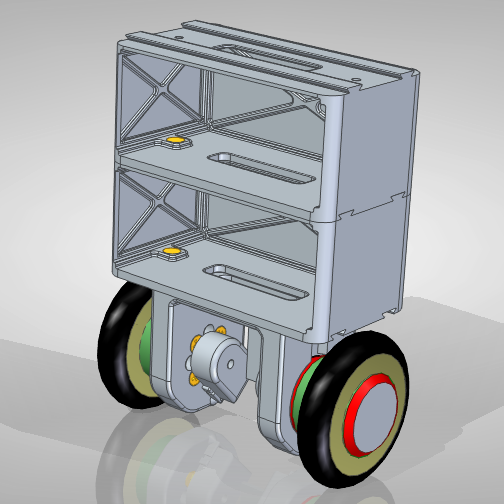
\includegraphics[width=0.5\textwidth]{images/gehaeuse-v2.png}
	% caption ist die Bildunterschrift, taucht auch im Abbildungsverzeichnis auf
	\caption{Gehäuse - V.2 \newline (Quelle: eigene Darstellung)}
	\label{gehaeuse-v2} % über das label kann man aus dem Text auf das Bild verweisen
\end{figure}
Im Bild \ref{gehaeuse-v2} ist eine modulare Darstellung des Roboters zu sehen. Das Motorhalter ist in diesem Fall als ein externer Modul dergestalt. Im ersten Modul von oben sollte man alle Steuerungsplatinen  einbauen. Das zweiten Modul von Oben sollte  das Akku beinhalten. Mit Hilfe vom Schwalbenschwanzverbindung und zwei Schrauben sollten die Module miteinander verbindet werden.

\subsection{Die Gehäusen - V.3}

Die Version V.2 (Bild \ref{gehaeuse-v2}) unterscheidet sich nicht viel von V.3. Es wurde die modulare Aufbau nicht geändert. Da hat man Schwalbenschwanzverbindung durch Steckverbindung ersetzt, die seitlich Zugeordnet sind. Es wurde auch Motorhalter modernisiert.

\begin{figure}[!h]  % [h] bedeutet, dass das Bild genau an dieser Stelle im Text erscheint
	% mit width=... wird die Größe des Bildes in Prozent der Seitenbreite eingestellt
	\centering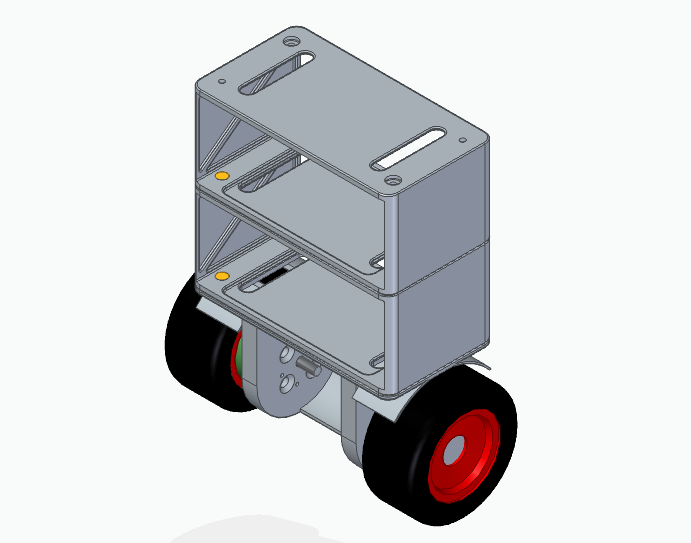
\includegraphics[width=0.5\textwidth]{images/gehaeuse-v3.png}
	% caption ist die Bildunterschrift, taucht auch im Abbildungsverzeichnis auf
	\caption{Gehäuse - V.2 \newline (Quelle: eigene Darstellung)}
	\label{gehaeuse-v3} % über das label kann man aus dem Text auf das Bild verweisen
\end{figure}

\subsection{Die Gehäusen - V.4}

Endgültige Gehäuse 

\begin{figure}[htb]
	\centering
	\begin{minipage}{0.45\linewidth}
		\centering
		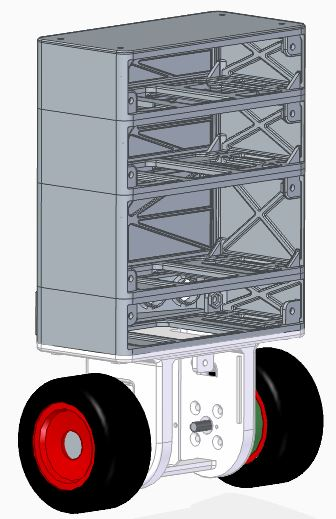
\includegraphics[scale=0.48]{images/4.1_vorne.jpg}
		\caption{Endgültige Gehäuse V4.1 \newline(Quelle: Eigene Darstellung)}
		\label{gehaeuse-v4}
	\end{minipage}
	%\hfill
	\begin{minipage}{0.45\linewidth}
		\centering
		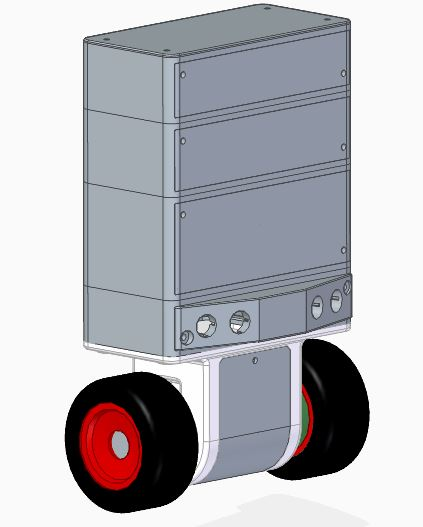
\includegraphics[scale=0.48]{images/4.1_hinten.jpg}
		\caption{ mit Deckels \newline (Quelle: Eigene Darstellung)}
	\end{minipage}
\end{figure}
\pagebreak
\subsection{Die Gehäusen - V.4.2.3}

Nach Zusammenbau des Roboters wurde folgende Korrektur noch durchgeführt:
 
\begin{itemize} 
	\item  mBed-Modul wurde 10 mm höher gemacht.
	\item  Anpassung an Kabelkanal Führung.
	\item  Beschriftung auf der Modulen.
	\item  Oberwand wurde komplett entfernt.
	\item  Versteifungen als Deckelsturzstelle.
	\item  Akku-Modul wurde 10 mm höher gemacht.
	\item  mBed und oDrive wurden stark nach einer Seite platziert.
\end{itemize}

\begin{figure}[htb]
	\centering
	\begin{minipage}{0.45\linewidth}
		\centering
		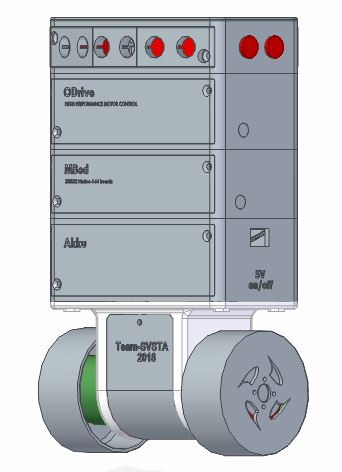
\includegraphics[scale=0.48]{images/V.4.3.jpg}
		\caption{Gehäuse V4.3 \newline(Quelle: Eigene Darstellung)}
		\label{gehaeuse-v4.3}
	\end{minipage}
	%\hfill
	\begin{minipage}{0.45\linewidth}
		\centering
		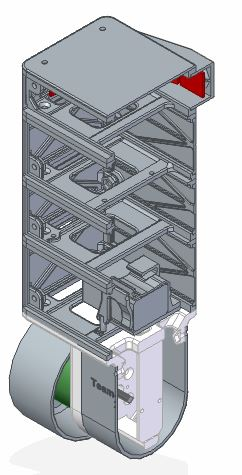
\includegraphics[scale=0.48]{images/V.4.3-1.jpg}
		\caption{ Schnitt \newline (Quelle: Eigene Darstellung)}
	\end{minipage}
\end{figure}
\pagebreak
\subsubsection{ Berechnung vom Motorhalter}
Alle Berechnungen wurden mit Hilfe von FEM - Programmierung gemacht und beweise die Festigkeit nur von dem Motorhalter. Es wurden an den Stellen vom Motoren und Räder das Moment laut der Berechnung \ref{FEM1} verwendet und als Lastkraft wurde 50N auf die Oberfläche eingeprägt.

Die Materialeigenschaften kann man aus der Abbildung \ref{FEM2} ablesen.

\begin{figure}[!h]  % [h] bedeutet, dass das Bild genau an dieser Stelle im Text erscheint
	\centering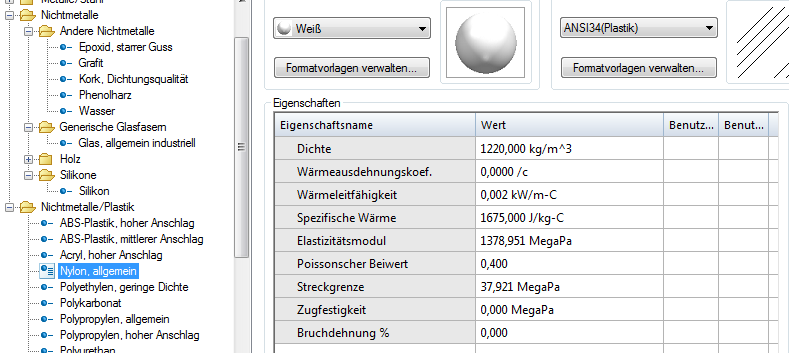
\includegraphics[width=0.7\textwidth]{images/FEM2.png}
	% caption ist die Bildunterschrift, taucht auch im Abbildungsverzeichnis auf
	\caption{Kunststoffeigenschaften - Nylon (PA) \newline (Quelle: eigene Darstellung)}
	\label{FEM2} % über das label kann man aus dem Text auf das Bild verweisen
\end{figure}
\begin{figure}[!h]  % [h] bedeutet, dass das Bild genau an dieser Stelle im Text erscheint
	% mit width=... wird die Größe des Bildes in Prozent der Seitenbreite eingestellt
	\centering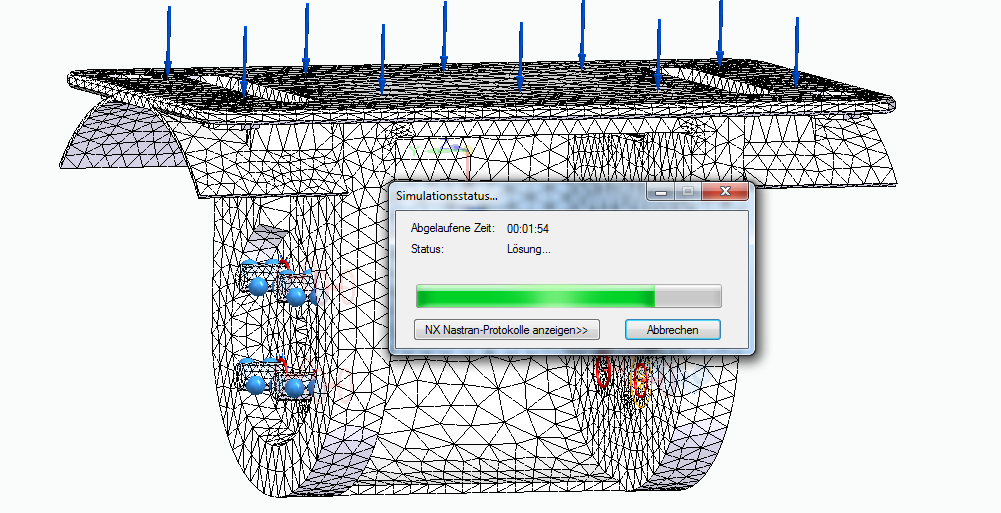
\includegraphics[width=0.9\textwidth]{images/FEM.png}
	% caption ist die Bildunterschrift, taucht auch im Abbildungsverzeichnis auf
	\caption{FEM-Berechnung \newline (Quelle: eigene Darstellung)}
	\label{FEM1} % über das label kann man aus dem Text auf das Bild verweisen
\end{figure}
\begin{figure}[!h]  % [h] bedeutet, dass das Bild genau an dieser Stelle im Text erscheint
	\centering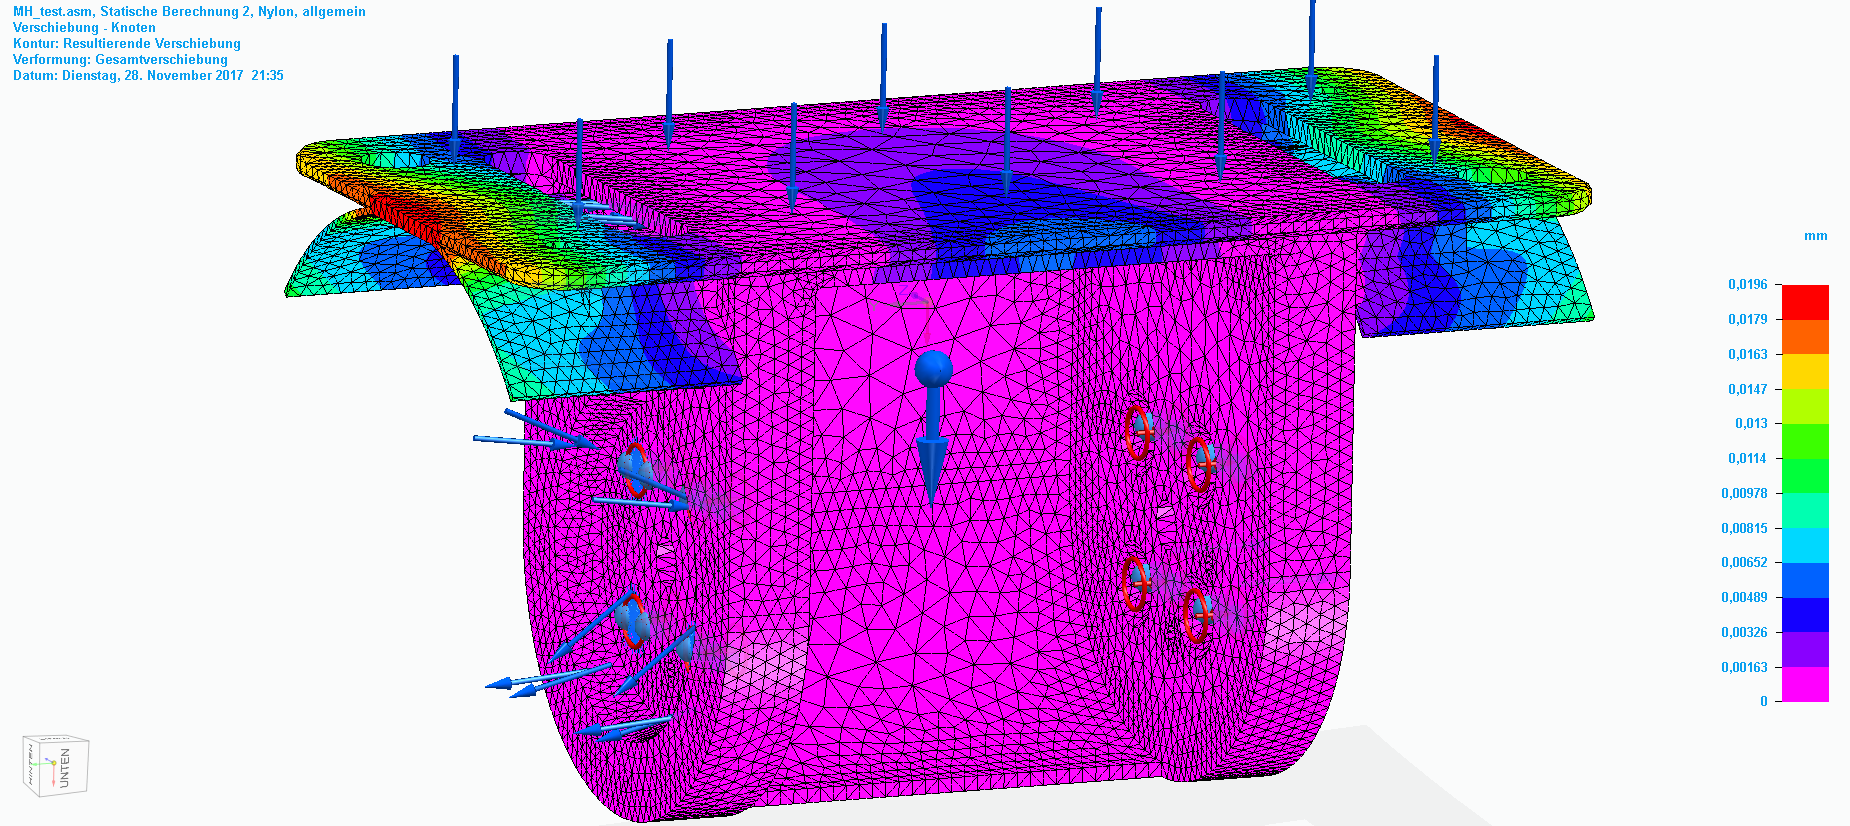
\includegraphics[width=0.9\textwidth]{images/FEM3.png}
	% caption ist die Bildunterschrift, taucht auch im Abbildungsverzeichnis auf
	\caption{FEM - Verschiebungen \newline (Quelle: eigene Darstellung)}
	\label{FEM3} % über das label kann man aus dem Text auf das Bild verweisen
\end{figure}
\pagebreak
Sicherheitsfaktor ....

\begin{figure}[!h]  % [h] bedeutet, dass das Bild genau an dieser Stelle im Text erscheint
	\centering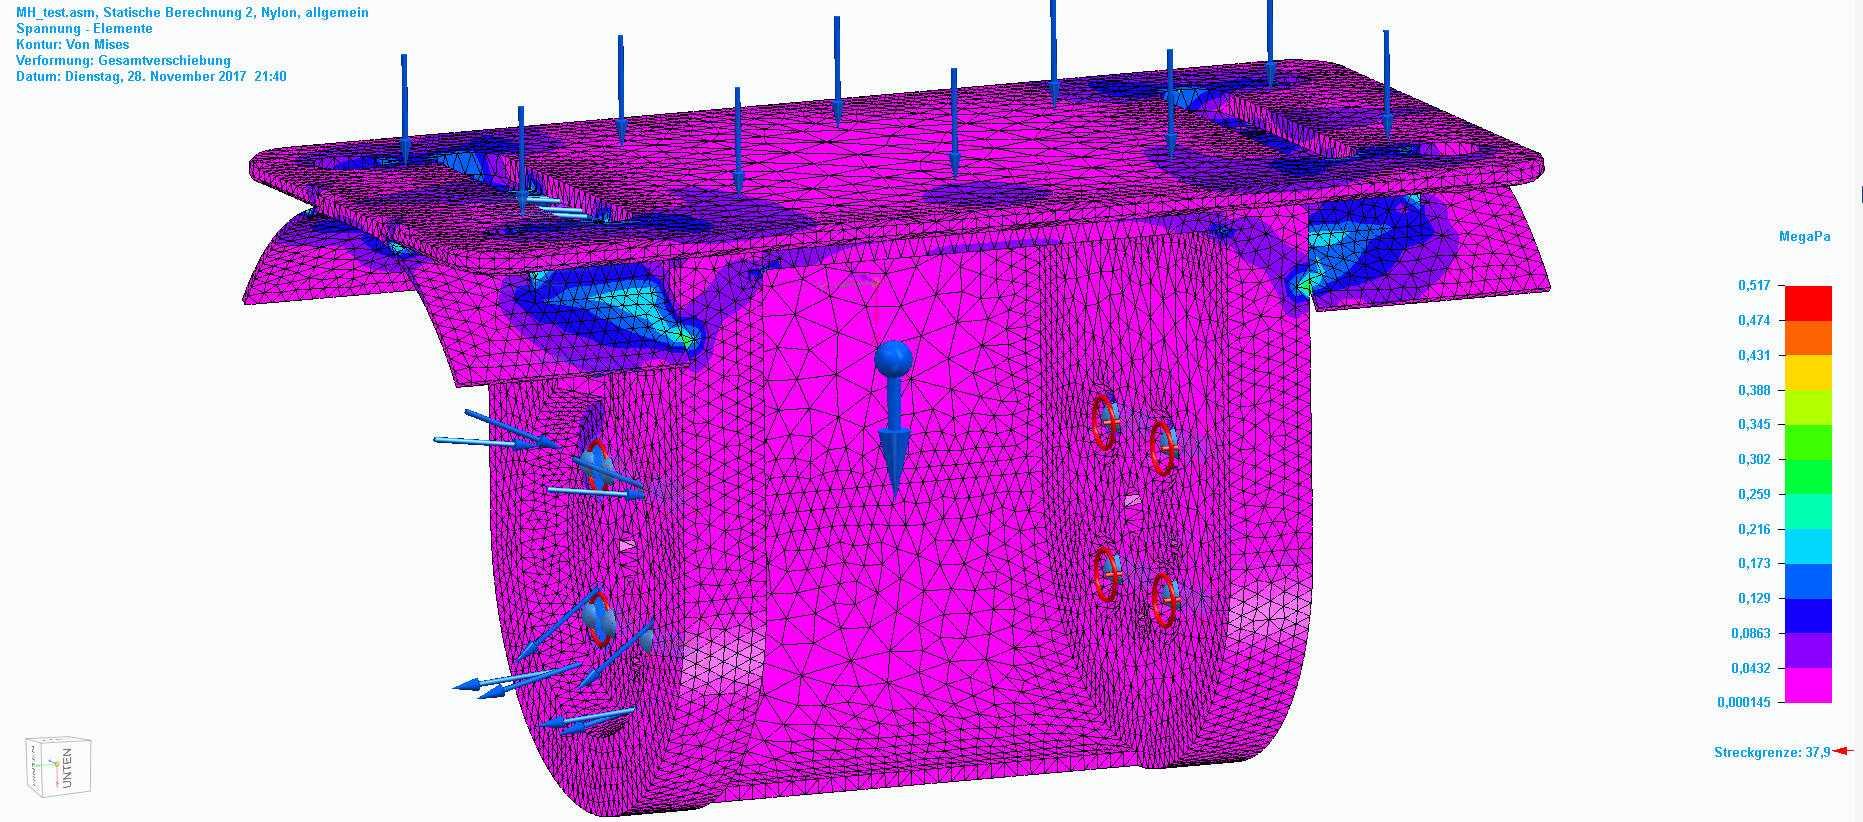
\includegraphics[width=0.9\textwidth]{images/FEM4.png}
	% caption ist die Bildunterschrift, taucht auch im Abbildungsverzeichnis auf
	\caption{FEM - Spannungen \newline (Quelle: eigene Darstellung)}
	\label{FEM4} % über das label kann man aus dem Text auf das Bild verweisen
\end{figure}
\pagebreak


% !TEX root = SegwayDoku.tex
\renewcommand{\autoren}{Valentyn Chepil}
\newpage
\section{Die ausgewählte Komponentenliste}
\subsection{Die Motoren}

% bild und Modul-Name

\subsection{Endcoder}

% bild und Modul-Name

\subsection{Driver}

% bild und Modul-Name

\subsection{Steuerungsplatine}

% bild und Modul-Name
Nucleo 

\subsection{Die Räder}

\begin{figure}[!h]  % [h] bedeutet, dass das Bild genau an dieser Stelle im Text erscheint
	% mit width=... wird die Größe des Bildes in Prozent der Seitenbreite eingestellt
	\centering\includegraphics[width=0.5\textwidth]{images/reifen.png}
	% caption ist die Bildunterschrift, taucht auch im Abbildungsverzeichnis auf
	\caption{Reifen \newline (Quelle: www.haertle.de )}
	\label{reifen} % über das label kann man aus dem Text auf das Bild verweisen
\end{figure}

quelle:
https://www.haertle.de/RC+Modellbau/RC+Car+Zubehoer/Reifen+Felgen+Raeder/TAMIYA+54188+DB+01+Dual+Block+Reifen+C+hinten+62+35.html
% bild
Felgen werden 3D moduliert und gedruckt. (In der Gruppe abfragen)

\subsection{Die Hinderniserkenner}

% bild und Modul-Name

US-Sensor und Infrarot-Sensor

\subsection{Bewegungs- und Beschleunigungsaufnehmer }

Hyroskop Modul-Name und Bild

\subsection{Netz (Akku)}

 Name und Bild
 
 \subsection{...}
 
 Name und Bild

